% ******************************* PhD Thesis Template **************************
% Please have a look at the README.md file for info on how to use the template

\documentclass[a4paper,12pt,oneside,times,numbered,print,index]{Classes/PhDThesisPSnPDF}

% ******************************************************************************
% ******************************* Class Options ********************************
% *********************** See README for more details **************************
% ******************************************************************************

% `a4paper'(The University of Cambridge PhD thesis guidelines recommends a page
% size a4 - default option) or `a5paper': A5 Paper size is also allowed as per
% the Cambridge University Engineering Deparment guidelines for PhD thesis
%
% `11pt' or `12pt'(default): Font Size 10pt is NOT recommended by the University
% guidelines
%
% `oneside' or `twoside'(default): Printing double side (twoside) or single
% side.
%
% `print': Use `print' for print version with appropriate margins and page
% layout. Leaving the options field blank will activate Online version.
%
% `index': For index at the end of the thesis
%
% `draftclassic': For draft mode without loading any images (same as draft in book)
%
% `draft': Special draft mode with line numbers, images, and water mark with
% timestamp and custom text. Position of the text can also be modified.
%
% `abstract': To generate only the title page and abstract page with
% dissertation title and name, to submit to the Student Registry
%
% `chapter`: This option enables only the specified chapter and it's references
%  Useful for review and corrections.
%
% ************************* Custom Page Margins ********************************
%
% `custommargin`: Use `custommargin' in options to activate custom page margins,
% which can be defined in the preamble.tex. Custom margin will override
% print/online margin setup.
%
% *********************** Choosing the Fonts in Class Options ******************
%
% `times' : Times font with math support. (The Cambridge University guidelines
% recommend using times)
%
% `fourier': Utopia Font with Fourier Math font (Font has to be installed)
%            It's a free font.
%
% `customfont': Use `customfont' option in the document class and load the
% package in the preamble.tex
%
% default or leave empty: `Latin Modern' font will be loaded.
%
% ********************** Choosing the Bibliography style ***********************
%
% `authoryear': For author-year citation eg., Krishna (2013)
%
% `numbered': (Default Option) For numbered and sorted citation e.g., [1,5,2]
%
% `custombib': Define your own bibliography style in the `preamble.tex' file.
%              `\RequirePackage[square, sort, numbers, authoryear]{natbib}'.
%              This can be also used to load biblatex instead of natbib
%              (See Preamble)
%
% **************************** Choosing the Page Style *************************
%
% `default (leave empty)': For Page Numbers in Header (Left Even, Right Odd) and
% Chapter Name in Header (Right Even) and Section Name (Left Odd). Blank Footer.
%
% `PageStyleI': Chapter Name next & Page Number on Even Side (Left Even).
% Section Name & Page Number in Header on Odd Side (Right Odd). Footer is empty.
%
% `PageStyleII': Chapter Name on Even Side (Left Even) in Header. Section Number
% and Section Name in Header on Odd Side (Right Odd). Page numbering in footer

% Uncomment to change page style
%\pagestyle{PageStyleII}

% ********************************** Preamble **********************************
% Preamble: Contains packages and user-defined commands and settings
% ******************************************************************************
% ****************************** Custom Margin *********************************

% Add `custommargin' in the document class options to use this section
% Set {innerside margin / outerside margin / topmargin / bottom margin}  and
% other page dimensions
\ifsetCustomMargin
  \RequirePackage[left=37mm,right=30mm,top=35mm,bottom=30mm]{geometry}
  \setFancyHdr % To apply fancy header after geometry package is loaded
\fi

% *****************************************************************************
% ******************* Fonts (like different typewriter fonts etc.)*************

% Add `customfont' in the document class option to use this section

\ifsetCustomFont
  % Set your custom font here and use `customfont' in options. Leave empty to
  % load computer modern font (default LaTeX font).
  \RequirePackage{helvet}
\fi

% *****************************************************************************
% **************************** Custom Packages ********************************

% ************************* Algorithms and Pseudocode **************************

%\usepackage{algpseudocode}


% ********************Captions and Hyperreferencing / URL **********************

% Captions: This makes captions of figures use a boldfaced small font.
%\RequirePackage[small,bf]{caption}

\RequirePackage[labelsep=space,tableposition=top]{caption}
\renewcommand{\figurename}{Fig.} %to support older versions of captions.sty


% *************************** Graphics and figures *****************************

%\usepackage{rotating}
%\usepackage{wrapfig}

% Uncomment the following two lines to force Latex to place the figure.
% Use [H] when including graphics. Note 'H' instead of 'h'
%\usepackage{float}
%\restylefloat{figure}

% Subcaption package is also available in the sty folder you can use that by
% uncommenting the following line
% This is for people stuck with older versions of texlive
%\usepackage{sty/caption/subcaption}
\usepackage{subcaption}

% ********************************** Tables ************************************
\usepackage{booktabs} % For professional looking tables
\usepackage{multirow}

%\usepackage{multicol}
%\usepackage{longtable}
%\usepackage{tabularx}


% ***************************** Math and SI Units ******************************

\usepackage{amsfonts}
\usepackage{amsmath}
\usepackage{amssymb}
\usepackage{siunitx} % use this package module for SI units


% ******************************* Line Spacing *********************************

% Choose linespacing as appropriate. Default is one-half line spacing as per the
% University guidelines

% \doublespacing
% \onehalfspacing
% \singlespacing


% ************************ Formatting / Footnote *******************************

% Don't break enumeration (etc.) across pages in an ugly manner (default 10000)
%\clubpenalty=500
%\widowpenalty=500

%\usepackage[perpage]{footmisc} %Range of footnote options


% *****************************************************************************
% *************************** Bibliography  and References ********************

%\usepackage{cleveref} %Referencing without need to explicitly state fig /table

% Add `custombib' in the document class option to use this section
\ifuseCustomBib
   \RequirePackage[square, sort, numbers, authoryear]{natbib} % CustomBib

% If you would like to use biblatex for your reference management, as opposed to the default `natbibpackage` pass the option `custombib` in the document class. Comment out the previous line to make sure you don't load the natbib package. Uncomment the following lines and specify the location of references.bib file

%\RequirePackage[backend=biber, style=numeric-comp, citestyle=numeric, sorting=nty, natbib=true]{biblatex}
%\bibliography{References/references} %Location of references.bib only for biblatex

\fi

% changes the default name `Bibliography` -> `References'
\renewcommand{\bibname}{References}


% *****************************************************************************
% *************** Changing the Visual Style of Chapter Headings ***************
% This section on visual style is from https://github.com/cambridge/thesis

% Uncomment the section below. Requires titlesec package.

%\RequirePackage{titlesec}
%\newcommand{\PreContentTitleFormat}{\titleformat{\chapter}[display]{\scshape\Large}
%{\Large\filleft{\chaptertitlename} \Huge\thechapter}
%{1ex}{}
%[\vspace{1ex}\titlerule]}
%\newcommand{\ContentTitleFormat}{\titleformat{\chapter}[display]{\scshape\huge}
%{\Large\filleft{\chaptertitlename} \Huge\thechapter}{1ex}
%{\titlerule\vspace{1ex}\filright}
%[\vspace{1ex}\titlerule]}
%\newcommand{\PostContentTitleFormat}{\PreContentTitleFormat}
%\PreContentTitleFormat


% ******************************************************************************
% ************************* User Defined Commands ******************************
% ******************************************************************************

% *********** To change the name of Table of Contents / LOF and LOT ************

%\renewcommand{\contentsname}{My Table of Contents}
%\renewcommand{\listfigurename}{My List of Figures}
%\renewcommand{\listtablename}{My List of Tables}


% ********************** TOC depth and numbering depth *************************

\setcounter{secnumdepth}{2}
\setcounter{tocdepth}{2}


% ******************************* Nomenclature *********************************

% To change the name of the Nomenclature section, uncomment the following line

%\renewcommand{\nomname}{Symbols}


% ********************************* Appendix ***********************************

% The default value of both \appendixtocname and \appendixpagename is `Appendices'. These names can all be changed via:

%\renewcommand{\appendixtocname}{List of appendices}
%\renewcommand{\appendixname}{Appndx}

% ******************************** Draft Mode **********************************

% Uncomment to disable figures in `draftmode'
%\setkeys{Gin}{draft=true}  % set draft to false to enable figures in `draft'

% These options are active only during the draft mode
% Default text is "Draft"
%\SetDraftText{DRAFT}

% Default Watermark location is top. Location (top/bottom)
%\SetDraftWMPosition{bottom}

% Draft Version - default is v1.0
%\SetDraftVersion{v1.1}

% Draft Text grayscale value (should be between 0-black and 1-white)
% Default value is 0.75
%\SetDraftGrayScale{0.8}


%% Todo notes functionality
%% Uncomment the following lines to have todonotes.

%\ifsetDraft
%	\usepackage[colorinlistoftodos]{todonotes}
%	\newcommand{\mynote}[1]{\todo[author=kks32,size=\small,inline,color=green!40]{#1}}
%\else
%	\newcommand{\mynote}[1]{}
%	\newcommand{\listoftodos}{}
%\fi

% Example todo: \mynote{Hey! I have a note}

\usepackage{float}
\usepackage{algorithm2e}
\usepackage[fontsize=13pt]{scrextend}
\usepackage{listings}
\usepackage {fancybox} 

\usepackage[utf8]{inputenc}
\usepackage[vietnamese,english]{babel}

\newenvironment{chapabstract}
{
  \begin{center} \large \bfseries Chapter Abstract \end{center}
  \list{}{
    \setlength{\leftmargin}{10mm}% <---------- CHANGE HERE
    \setlength{\rightmargin}{\leftmargin}%
  }%
  \item \itshape \relax
  \endlist
}
{\par \vspace*{5mm}}

\makeatother

% ************************ Thesis Information & Meta-data **********************
% Thesis title and author information, refernce file for biblatex
% ************************ Thesis Information & Meta-data **********************
%% The title of the thesis
\title{Malware Detection using Machine Learning in Windows operation systems}
%\texorpdfstring is used for PDF metadata. Usage:
%\texorpdfstring{LaTeX_Version}{PDF Version (non-latex)} eg.,
%\texorpdfstring{$sigma$}{sigma}

%% Subtitle (Optional)
% \subtitle{Using the CUED template}

%% The full name of the author
\author{Pham Huu Danh}

%% Department (eg. Department of Engineering, Maths, Physics)
\dept{Faculty of Software Engineering}

%% University and Crest
\university{University of Infomation Technology}
% Crest minimum should be 30mm.
\crest{
\includegraphics[width=0.2\textwidth]{UIT_Logo}}
%% Use this crest, if you are using the college crest
%% Crest long miminum should be 65mm
%\crest{\includegraphics[width=0.45\textwidth]{University_Crest_Long}}

%% College shield [optional] 
% Crest minimum should be 30mm.
%\collegeshield{\includegraphics[width=0.2\textwidth]{CollegeShields/Kings}}


%% Supervisor (optional)
%% for multiple supervisors, append each supervisor with the \newline command
\supervisor{Assoc Prof. Dr. Vu Thanh Nguyen}

%% Supervisor Role (optional) - Supervisor (default) or advisor
% \supervisorrole{\textbf{Supervisors: }}
%% if no title is desired:
% \supervisorrole{}

%% Supervisor line width: required to align supervisors
%\supervisorlinewidth{0.35\textwidth}

%% Advisor (optional)
%% for multiple advisors, append each advisor with the \newline command
%\advisor{Dr. A. Advisor\newline
%Dr. B. Advisor}
     
%% Advisor Role (optional) - Advisor (default) or leave empty
% \advisorrole{Advisors: }
%% if no title is required
% \advisorrole{}

%% Advisor line width: required to align supervisors
%\advisorlinewidth{0.25\textwidth}


%% You can redefine the submission text:
% Default as per the University guidelines:
% ``This dissertation is submitted for the degree of''
%\renewcommand{\submissiontext}{change the default text here if needed}

%% Full title of the Degree
\degreetitle{Bachelor of Software Engineering}

%% College affiliation (optional)
% \college{King's College}

%% Submission date
% Default is set as {\monthname[\the\month]\space\the\year}
\degreedate{June 2018} 

%% Meta information
\subject{Malware Detection using Machine Learning in Windows operation systems} \keywords{{UIT}{ Undergraduate Thesis} {Engineering} {University of
Information Techonology} {Malware Detection} {Machine Learning}}

% ***************************** Abstract Separate ******************************
% To printout only the titlepage and the abstract with the PhD title and the
% author name for submission to the Student Registry, use the `abstract' option in
% the document class.

\ifdefineAbstract
 \pagestyle{empty}
 \includeonly{Declaration/declaration, Abstract/abstract}
\fi

% ***************************** Chapter Mode ***********************************
% The chapter mode allows user to only print particular chapters with references
% Title, Contents, Frontmatter are disabled by default
% Useful option to review a particular chapter or to send it to supervisior.
% To use choose `chapter' option in the document class

\ifdefineChapter
 \includeonly{
  Chapter2/chapter2,
  Chapter4/chapter4,
  Chapter5/chapter5
 }
\fi

% ******************************** Front Matter ********************************
\begin{document}

\frontmatter

% \maketitle
\pdfbookmark[0]{Cover}{label:cover-page}%
\begin{titlepage}

\newgeometry{top=15mm,bottom=30mm,left=5mm,right=30mm,
hmarginratio=1:1,vmarginratio=1:1,bindingoffset=5mm}

\thisfancypage{
\setlength{\fboxrule}{2pt}
\setlength{\fboxsep}{15pt}
\doublebox
}{}

% \begin{changemargin}{-35mm}{-20mm}

\begin{center}
  
\textbf{\large VIETNAM NATIONAL UNIVERSITY HO CHI MINH CITY} \\[2mm]
\textbf{\Large UNIVERSITY OF INFORMATION TECHNOLOGY} \\ [2mm]
\textbf{\Large FACULTY OF SOFTWARE ENGINEERING}

\vspace{0.1\textheight}
\begin{otherlanguage}{vietnamese}
\textbf{\large PHẠM HỮU DANH}
\end{otherlanguage}

\vspace{0.1\textheight}
\textbf{\Large BACHELOR’S THESIS} \\ [10mm]

\textbf{\Large MALWARE DETECTION USING MACHINE } \\ [2mm]
\textbf{\Large LEARNING IN WINDOWS OPERATING SYSTEMS } \\ [10mm]

\begin{otherlanguage}{vietnamese}
\textbf{ \Large PHÁT HIỆN MÃ ĐỘC BẰNG PHƯƠNG PHÁP } \\ [2mm]
\textbf{ \Large MÁY HỌC TRÊN HỆ ĐIỀU HÀNH WINDOWS }
\end{otherlanguage}

\vspace{0.15\textheight}

\textbf{\large BACHELOR OF SCIENCE IN SOFTWARE ENGINEERING}

\vspace{\fill}
\textbf{\large HO CHI MINH CITY, 2018}
\end{center}

% \end{changemargin}
\end{titlepage}
\cleardoublepage


\begin{titlepage}

\newgeometry{top=15mm,bottom=30mm,left=25mm,right=25mm,
hmarginratio=1:1,vmarginratio=1:1,bindingoffset=5mm}
\thisfancypage{
    \setlength{\fboxsep}{15pt}
    \doublebox
}{}

\begin{center}
  
\textbf{\large VIETNAM NATIONAL UNIVERSITY HO CHI MINH CITY} \\[2mm]
\textbf{\Large UNIVERSITY OF INFORMATION TECHNOLOGY} \\ [2mm]
\textbf{\Large FACULTY OF SOFTWARE ENGINEERING}

\vspace{0.07\textheight}
\begin{otherlanguage}{vietnamese}
\textbf{\large PHẠM HỮU DANH - 14520134}
\end{otherlanguage}

\vspace{0.1\textheight}
\textbf{\Large BACHELOR’S THESIS} \\ [10mm]

\textbf{\Large MALWARE DETECTION USING MACHINE } \\ [2mm]
\textbf{\Large LEARNING IN WINDOWS OPERATING SYSTEMS} \\ [10mm]
\begin{otherlanguage}{vietnamese}
\textbf{ \Large PHÁT HIỆN MÃ ĐỘC BẰNG PHƯƠNG PHÁP} \\ [2mm]
\textbf{ \Large MÁY HỌC TRÊN HỆ ĐIỀU HÀNH WINDOWS}
\end{otherlanguage}

\vspace{0.1\textheight}
\textbf{\large BACHELOR OF SCIENCE IN SOFTWARE ENGINEERING} 

\vspace{0.07\textheight}
\textbf{\large SUPERVISOR} \\ [2mm]
\begin{otherlanguage}{vietnamese}
\textbf{\large ASSOC PROF. DR. VŨ THANH NGUYÊN}
\end{otherlanguage}


\vspace{\fill}
\textbf{\large HO CHI MINH CITY, 2018}

\end{center}
\end{titlepage}
\cleardoublepage


% \include{Dedication/dedication}
% include{Declaration/declaration}
% ************************** Thesis Acknowledgements *****************************

\begin{acknowledgements}      

% ************************** Thesis Acknowledgements *****************************
Đầu tiên và trên hết, tôi xin gửi lời cảm ơn chân thành nhất đến giảng viên, PGS. TS. Vũ Thanh Nguyên. Tôi chân thành biết ơn và cảm ơn thầy vì những chỉ dẫn vô giá, những hướng dẫn giá trị và những động lực từ tinh thần nghiên cứu liên tục của thầy. Những kinh nghiệm và sự giảng dạy của thầy trong lĩnh vực khóa học máy tính nói chung, và công nghệ phần mềm nói riêng, tôi có được những kiến thức mới, đầy giá trị và niềm đam mê trong lĩnh vực máy học và nhận dạng mã độc. Thầy là nguồn cảm hứng của tôi qua những trở ngại trong thời gian làm khóa luận tốt nghiệp. Nếu không có sự giúp đỡ của thầy, tôi sẽ không thể hoàn thành khóa luận này.

Tôi cũng gửi lời cảm ơn đến thầy Huỳnh Nguyễn Khắc Huy để về sự hướng dẫn của thầy về học máy và bảo mật máy tính.

Tôi cũng biết ơn tất cả các giảng viên của khoa Kỹ thuật Phần mềm tại trường Đại học Công nghệ Thông tin. Nhờ sự cống hiến của họ, tôi có một nền tảng vững chắc về khoa học máy tính nói chung và kiến thức về công nghệ phần mềm nói riêng. Nhờ các thầy cô, tôi học được khả năng học hỏi và áp dụng các công nghệ mới một cách hiệu quả hơn.

Cuối cùng nhưng không kém phần quan trọng, tôi xin cảm ơn gia đình đã khuyến khích và hỗ trợ tài chính lúc tôi cần. Tôi mãi mãi biết ơn tình yêu vô điều kiện của họ.

\end{acknowledgements}

% ************************** Thesis Abstract *****************************
% Use `abstract' as an option in the document class to print only the titlepage and the abstract.
\renewcommand{\abstractname}{Executive Summary}

\begin{abstract}
Static malware detection is an essential layer in a security suite, which attempts to classify samples as malicious or benign before execution. 
However, most of the related works incur the scalability issues, for examples, methods using neural networks usually take a lot of training time \cite{raff2017malware}, or use imbalanced datasets \cite{saxe2015deep,vu2017metamorphic}, which makes validation metrics misleading in reality.

In this study, we research the two essential approaches for malware detection (i.e., static and dynamic analysis) and conduct experiments to apply the machine learning methods in static malware detection. 
Furthermore, we propose a static malware detection method by Portable Executable analysis and Gradient Boosting Decision Tree algorithm. 
We manage to reduce the training time by appropriately reducing the feature dimension. 
The experiment results show that our proposed method can achieve up to 99.394\% detection rate at 1\% false alarm rate, and score results in less than 0.1\% false alarm rate at a detection rate 97.572\%, based on more than 600,000 training and 200,000 testing samples from Endgame Malware BEnchmark for Research (EMBER) dataset \cite{anderson2018ember}.
\end{abstract}


% *********************** Adding TOC and List of Figures ***********************

\tableofcontents

\listoffigures

\listoftables

% \printnomenclature[space] space can be set as 2em between symbol and description
%\printnomenclature[3em]

\printnomenclature

% ******************************** Main Matter *********************************
\mainmatter

%*******************************************************************************
%*********************************** First Chapter *****************************
%*******************************************************************************

\chapter{MỞ ĐẦU}
\label{chap:problem-statement}
\graphicspath{{Chapter1/Figs/}}

\begin{chapabstract}
{Chương \ref{chap:problem-statement} đặt vấn đề cho đề tài, bao gồm sự nguy hiểm của phần mềm độc hại, tổng quan về tình hình nghiên cứu, ứng dụng các phương pháp máy học vào nhận diện mã độc, và đặc biệt là trình bày những hạn chế của các phương pháp đã có, cũng chính là lí do của việc chọn đề tài.}
\end{chapabstract}
Malware thường được sử dụng như một thuật ngữ chung để chỉ bất kỳ phần mềm nào được thiết kế nhằm mục đích gây thiệt hại cho một máy tính, máy chủ hoặc mạng máy tính \cite{moir2003defining}. 
Một sự cố từ malware có thể gây thiệt hại hàng triệu đô la, cụ thể, mã độc zero-day ransomware WannaCry đã gây ra thảm họa trên toàn thế giới từ việc đánh sập hệ thống của các Bệnh viện Dịch vụ Y tế Quốc gia Vương quốc Anh, cho đến việc tắt toàn bộ hệ thống sản xuất của công ty Honda tại Nhật Bản \cite{chen2017automated}.
Hơn nữa, phần mềm độc hại ngày càng trở nên tinh vi và đa dạng hơn mỗi ngày \cite{shahi2009technology}. Theo đó, bài toán phát hiện phần mềm độc hại là một vấn đề quan trọng trong an ninh mạng, đặc biệt khi xã hội trở nên phụ thuộc nhiều vào các hệ thống máy tính.

Các sản phẩm nhận diện malware trước đó thường sử dụng các phương pháp dựa trên quy tắc (rule-based) hoặc dựa trên chữ ký (signature-based), yêu cầu các nhà phân tích xử lý các quy tắc thủ công (handcraft rules) có liên quan để phát hiện mã độc.
Cách tiếp cận này có độ chính xác cao.
Tuy nhiên, các quy tắc này  thường là cụ thể và không thể nhận ra phần mềm độc hại mới, ngay cả khi nó sử dụng cùng chức năng.
Vì lý do này, ý tưởng phát hiện mã độc dựa trên các thuật toán học máy được phát sinh.
Thuật toán học máy học các mẫu cơ bản (pattern) từ một tập huấn luyện nhất định, bao gồm cả các mẫu độc hại và lành tính.
Những pattern phân biệt các phần mềm độc hại từ phần mềm lành tính.
Kể từ khi Schultz và các cộng sự chó thấy sự hiệu quả của việc ứng dụng các thuật toán máy học vào nhận diện mã độc \cite{schultz2001data}, máy học đang trở thành một trong những công cụ phổ biến và có nhiều ảnh hưởng trong việc đảm bảo an toàn cho hệ thống.

Một số phương pháp sử dụng học máy đã mang lại các mô hình quá tích cực, thể hiện độ chính xác dự báo đáng kể, nhưng đã dẫn đến nhiều những kết quả dương tính giả (false positives). Các kết quả dương tính giả làm tiêu cực trải nghiệm của người dùng, ngăn không cho triển khai các phần mềm mới. Theo khảo sát của các IT administrator năm 2017 \cite{jonathan2017survey}, 42\% các công ty cho rằng người dùng của họ bị mất năng suất là do liên quan đến những kết quả dương tính giả, tạo ra một điểm nghẹt cho các quản trị viên CNTT trong môi trường doanh nghiệp. Các kỹ sư bảo mật cũng thông báo các báo động giả này thường gây rối khi họ đang làm việc để phát hiện và loại bỏ phần mềm độc hại.
Một báo cáo được công bố vào năm 2015 cũng cho thấy rằng nhiều tổ chức ở Hoa Kỳ đã tiêu thụ một lượng tiền khổng lồ để xử lý các cảnh báo phần mềm độc hại không chính xác \cite{eduard2015false}. Do đó, ngay cả khi một giải pháp có tỷ lệ phát hiện cao nhất, nếu nó có một số lượng lớn các kết quả dương tính giả, nó được xem là vô dụng hơn so với một giải pháp với các kết quả dương tính giả thấp và một tỷ lệ phát hiện vừa phải.

Chúng tôi chọn đề tài "Phát hiện Mã độc nằng phương pháp Máy học trên hệ điều hành Windows" với mong muốn đóng góp một phương pháp mới để giải quyết vấn đề xác định phần mềm độc hại, đạt được tỷ lệ phát hiện cao và tỷ lệ dương giả thấp.

%*******************************************************************************
%****************************** Second Chapter *********************************
%*******************************************************************************

\chapter{Introduction}
\label{chap:introduction}
\graphicspath{{Chapter2/Figs/}}

\begin{chapabstract}
Chapter \ref{chap:introduction} presents the overview of applying Machine Learning in Static Malware Detection on Windows operating systems; the motivation and the objectives of the thesis; list the related researches of authors either in Viet Nam or over the world; and the background.
\end{chapabstract}

\section{Overview}
\label{sec:overview}

Malware is software designed to infiltrate or harm a computer system without the owner's informed consent (section \ref{sec:malware}). A simple classification of malware is the recognizing malware files and clean files. Static malware detection is classifying samples as malicious or benign without executing them, in contrast to dynamic malware detection which detects malware based on its runtime behavior \cite{athiwaratkun2017malware, dahl2013large}. Although static malware detection is well-known to be undecidable in general \cite{cohen1987computer}, it is a critical layer in a security suite because when successful, it allows identifying malicious files before execution.

Besides, machine learning is an attractive tool for either a first detection capability or additional detection heuristics (section \ref{ssec:machine-learning-intro}). Supervised learning models automatically find out complex relationships between file attributes in training data that are distinguishing between malicious and benign samples (section \ref{ssec:supervised-learning}). Moreover, machine learning models generalize to new dataset whose features and labels follow a similar pattern to the training data. 

Additionally, in Windows operating systems, the general format for malware is Portable Executable (PE) format (section \ref{sec:pe-file}), which is the file format for executables, object code, DLLs, FON Font files, and others used in both 32-bit and 64-bit versions. The PE format encapsulates the information necessary for the Windows operating system loader to manage the wrapped executable code.

Therefore, various machine learning-based static Portable Executable (PE) malware detectors have been proposed since at least 1995 \cite{kephart1995biologically}. Schultz et al. \cite{schultz2001data} represented PE files by features that included imported functions, strings, and byte sequences. Models included rules induced from RIPPER \cite{cohen1995fast}, Naive Bayes and an ensemble classifier. This approach was extended by Kolter et al. \cite{kolter2006learning} by including byte-level N-grams and techniques from natural language processing, including TFIDF weighting of strings. Shafiq et al. \cite{Shafiq2009AFF} proposed using just seven features from the PE header, driven by the fact that most malware applications in their study typically presented those elements. Saxe and Berlin used two-dimensional byte entropy histograms and a multi-layer neural network for classification \cite{saxe2015deep}.

\section{Motivation}
\label{sec:motivation}

Although many models have performed prominent predictive accuracy, they were trained and validated on an imbalanced dataset because malware detection has not received the same attention in the open research community as other applications, where rich benchmark datasets exist. Legal restrictions are the primary challenge for releasing a benchmark dataset for malware detection, i.e., Saxe and Berlin are not able to release the data or code for their project due to its legal and proprietary nature \cite{saxe2015deep}. Additionally, unlike images, text and speech which may be labeled approximately instantly, and in many cases by a non-expert determining, whether a binary file is malicious or benign can be a time-consuming process for even the well-trained. The work of labeling may be automated via anti-malware, but the results may be proprietary or otherwise protected. Hence, these models may not impress with balanced data \cite{chawla2009data}.

Furthermore, a productive method, which has impressive accuracy and very-low false positive rate, prevents the massive losses from malware, also gives a pleasant user experience and save resources for many organizations.

\section{Objectives}
\label{sec:objectives}

As mentioned in section \ref{sec:motivation}, the result from many proposed approaches may not be impressive when evaluating with balanced data. Since the \textbf{primary objective} of this thesis is to \textbf{apply the machine learning methods in malware detection with an balanced dataset}. Additionally, the \textbf{expected objective} is to propose an method with \textbf{a high detection rate} and \textbf{an extremely low false alarm rate}. Ultimately, we aim the knowledge of machine learning and how to apply them to enhance the user information security in solving the malware detection problem. The detailed work that  we have done in this thesis includes:
\begin{itemize}
\item Study and build the background in information security, especially malware.
\item Study and understand the fundamental knowledge in Machine  Learning including classification, decision tree algorithm, random forest algorithm, support vector machine algorithm, neural networks, and gradient-boosting decision tree algorithm. 
\item Research and gain a detailed understanding of the gradient-boosting decision tree algorithm.
\item Apply gradient-boosting decision tree algorithm in malware detection. Conduct some experiments to evaluate the performance of the model and optimize the parameters.
\item Build a demo application with Windows ML which is the new platform released with Windows 10 April 2018 Update.
\end{itemize}

\section{Related Works}

Malware detection has grown over the past several years, due to the more rising threat posed by malware to large businesses and governmental agencies. In Viet Nam, there are various public researches about malware detection and applying machine learning in malware detection. For examples, Assoc Prof. Dr. Vu Thanh Nguyen et al. proposed a combined approach of Negative Selection Algorithm and Artificial Immune Network for virus detection \cite{nguyen2014combination}, and the method for the metamorphic malware detection by Portable Executable (PE) Analysis with the Longest Common Sequence (LCS) \cite{vu2017metamorphic}; Dr. Van-Hau Pham, Nguyen Tan Cam and Ly Hoang Tuan published many researches related to malware detection in Android operating system \cite{pham2017eddleak, cam2017sensitive, tuan2017enhancing}; Nguyen Van Nhuong et al. proposed a semantic set method to detect metamorphic malware effectively \cite{van2014semantic}.

Traditionally, the two essential approaches for malware detection can be approximately split based on the method that is used to analyze the malware, either static and dynamic analysis \cite{egele2012survey}.

In theory, dynamic detection provides the direct view of malware action, is less vulnerable to obfuscation, and makes it harder to reuse existing malware \cite{moser2007limits}. However, in practice, malware can identify if it is running in a sandbox, prevent itself from performing the malicious behavior \cite{vidas2014evading}. This resulted in an arms race between dynamic behavior detectors and malware. Further, in many cases, malware does not execute correctly, due to missing dependencies or unexpected system configuration. These issues make it difficult to collect a dataset of malware behavior. Additional, in many cases, malware does not execute correctly, due to missing dependencies or unexpected system configuration.  These issues make it difficult to collect a dataset of malware behavior.

In contrast, static analysis, is widely known to be undecidable \cite{cohen1987computer}, does not require complicated or expensive setup for gathering, and has enormous datasets can be created by aggregating the binaries files. These reasons make static malware detection very responsive to machine learning approaches, which tends to perform better as data size increases \cite{banko2001scaling}.

As mentioned in section \ref{sec:overview}, several machine learning-based static malware detection programs have been introduced since at least 1995 \cite{kephart1995biologically}. Numerous static features have been proposed for extracting  features  from  binaries:  printable  strings \cite{schultz2001data}, import tables, opcodes, informational entropy, \cite{weber2002toolkit}, byte n-grams \cite{abou2004n}, two dimensional byte entropy histograms \cite{saxe2015deep}. Many other features have also been suggested during the Microsoft Malware Classification Challenge on Kaggle \cite{ronen2018microsoft}, such as opcode images, various decompiled assembly features, and aggregate statistics. In additional, inspired by the success of end-to-end deep learning models in image processing and natural language processing, Raff et al. introduced malware detection from raw byte sequences \cite{raff2017malware}. Maybe the state-of-the-art models will change to end-to-end deep learning models in the ensuing months or years, but hand-crafted features may continue to be relevant because of the structured format of malware.

The feature space can become large, in those cases methods like locality-sensitive hashing \cite{bayer2009scalable}, feature hashing \cite{jang2011bitshred} or random projections \cite{fradkin2003experiments} have been applied in malware detection.

Even after applying dimensionality reduction, there is still a large number of features, which can cause scalability issues for some machine learning algorithms, e.g., Support Vector Machine (SVM) and k-nearest neighbors (k-NN). Lately, neural networks have emerged as a scalable alternative due to significant advances in training algorithm \cite{almasi2016review}. Many approaches using neural networks have been introduced \cite{saxe2015deep, dahl2013large, kephart1995biologically, benchea2014combining} though it is not explicit how to compare results because of different datasets.

Another popular alternative is the ensemble of trees, which can scale reasonably efficiently by subsampling the feature space during each iteration \cite{breiman2001random}. Decision trees can adapt well to various data types and are flexible to multiple scales of values in feature vectors, so they give good performance even without some data standardization.


\chapter{Background}
\label{chap:background}
\graphicspath{{Chapter3/Figs/}}

\begin{chapabstract}
Firstly, chapter \ref{chap:background} presents the theoretical background used in the thesis including malware types, PE file format and academic background in machine learning. Then, machine learning frameworks and tools are introduced to reveal our implementation in practice.
\end{chapabstract}

\section{Malware Types}
\label{sec:malware}

Classifying is the excellent way to have a better understanding of malware. There are several of the most common types: adware, bots, rootkits, spyware, Trojan horses, viruses, and worms \cite{neil2012common}.

\subsection{Virus}

A virus is a form of malware that is capable of replicating itself and spreading to other computers by attaching themselves to various applications and executing when a user launches one of those. Viruses can also spread through documents, script files, and cross-site scripting vulnerabilities in web apps. Some famous examples of viruses over the years are the Concept virus, the Chernobyl virus (also known as CIH), the Anna Kournikova virus, Brain, and RavMonE.exe.

\subsection{Worm}

A worm is a standalone software that replicates without targeting and infecting specific files. Think of worms as small programs that replicate themselves and destroy the data. They usually aim the operating system files and work until the drive they are in becomes empty. Some examples include Melissa, Morris, Mydoom, Sasser, and Blaster.

\subsection{Trojan}

A Trojan is a malicious application that misrepresents itself to look useful to fool users into downloading and installing. A trojan can give remote access to an infected computer which is possible for the attacker to steal data, install more malware, monitor user activity, etc. Notable examples also include Trojan horses developed by United States government agencies like the FBI and NSA. Names like Magic Lantern, FinFisher, Netbus, Beast, Gh0st RAT, Clickbot.A, and Zeus have been the reason of horror. While an Android malware discovered in 2015, called Shedun, is one of the many that target mobile devices.

\subsection{Ransomware}

Ransomware, which is one of the most advanced and continuously on the rise these days, is a kind of malware that typically holds a computer system captive while requiring a ransom, e.g., blocking the access to the data of a victim or threating to either publish it. Worse yet, there is no guarantee that paying will get access to the data, or prevent it from publishing. Major ransomware like Reveton, CryptoLocker, CryptoWall, and more recently, the 2017 WannaCry attack, have caused no small amount of destruction \cite{chen2017automated}.

\subsection{Rootkit}

A rootkit is a collection of software specially designed to allow malware that gathers information, into your system. These work in the background so that a user may not notice anything different. But in the environment, a rootkit will permit several types of malware to get into the system. The first rootkit to gain reputation on Windows was NTRootkit in 1999, but the most popular is the Sony BMG copy protection rootkit scandal that shook the company in the year 2005 \cite{bruce2005sony}.

\subsection{Adware}

Although the advertising-supported software (adware) is now much more common and known as adware in some circles, this word has been linked to malware for quite some time. While adware can refer to any application that is supported by advertising, malicious adware usually displays ads in the form of popups and windows that cannot be closed. It is the perhaps the most productive and least dangerous malware, designed with the specific purpose of promoting ads on your computer.

\subsection{Bot}

Bots are software programs created to perform specific operations automatically. While some bots are created for approximately innocent purposes, it is becoming increasingly common to see bots being used maliciously. Bots can be used in botnets (collections of machines to be controlled by third parties) to perform distributed denial of service attacks, send spam, and steal data.

\section{PE File Format}
\label{sec:pe-file}

The Portable Executable (PE) file format describes the predominant executable format for Microsoft Windows operating systems and includes executables, dynamically-linked libraries (DLLs), and FON font files. The format is currently supported on Intel, AMD, and variants of ARM instruction set architectures.

A Portable Executable file consists of some headers and sections that tell the dynamic linker how to map the file into memory. An executable image includes of several different regions, each of which requires different memory protection; so the start of each section must be aligned to a page frame. Typically, headers include the Common Object File Format (COFF) file header that contains essential information such as the type of machine for which the file is intended, the nature of the file (DLL, EXE, OBJ), the number of sections, the number of symbols, etc. The optional header identifies the linker version, the size of the code, the size of initialized and uninitialized data, the address of the entry point, etc. Data directories within the optional header provide pointers to the sections that follow it. These sections include tables for exports, imports, resources, exceptions, debug information, certificate information, and relocation tables. So, it provides a useful summary of the contents of an executable \cite{shafiq2009pe}. Finally, the section table outlines the name, offset and size of each section in the PE file.

\begin{figure}[H] 
\centering    
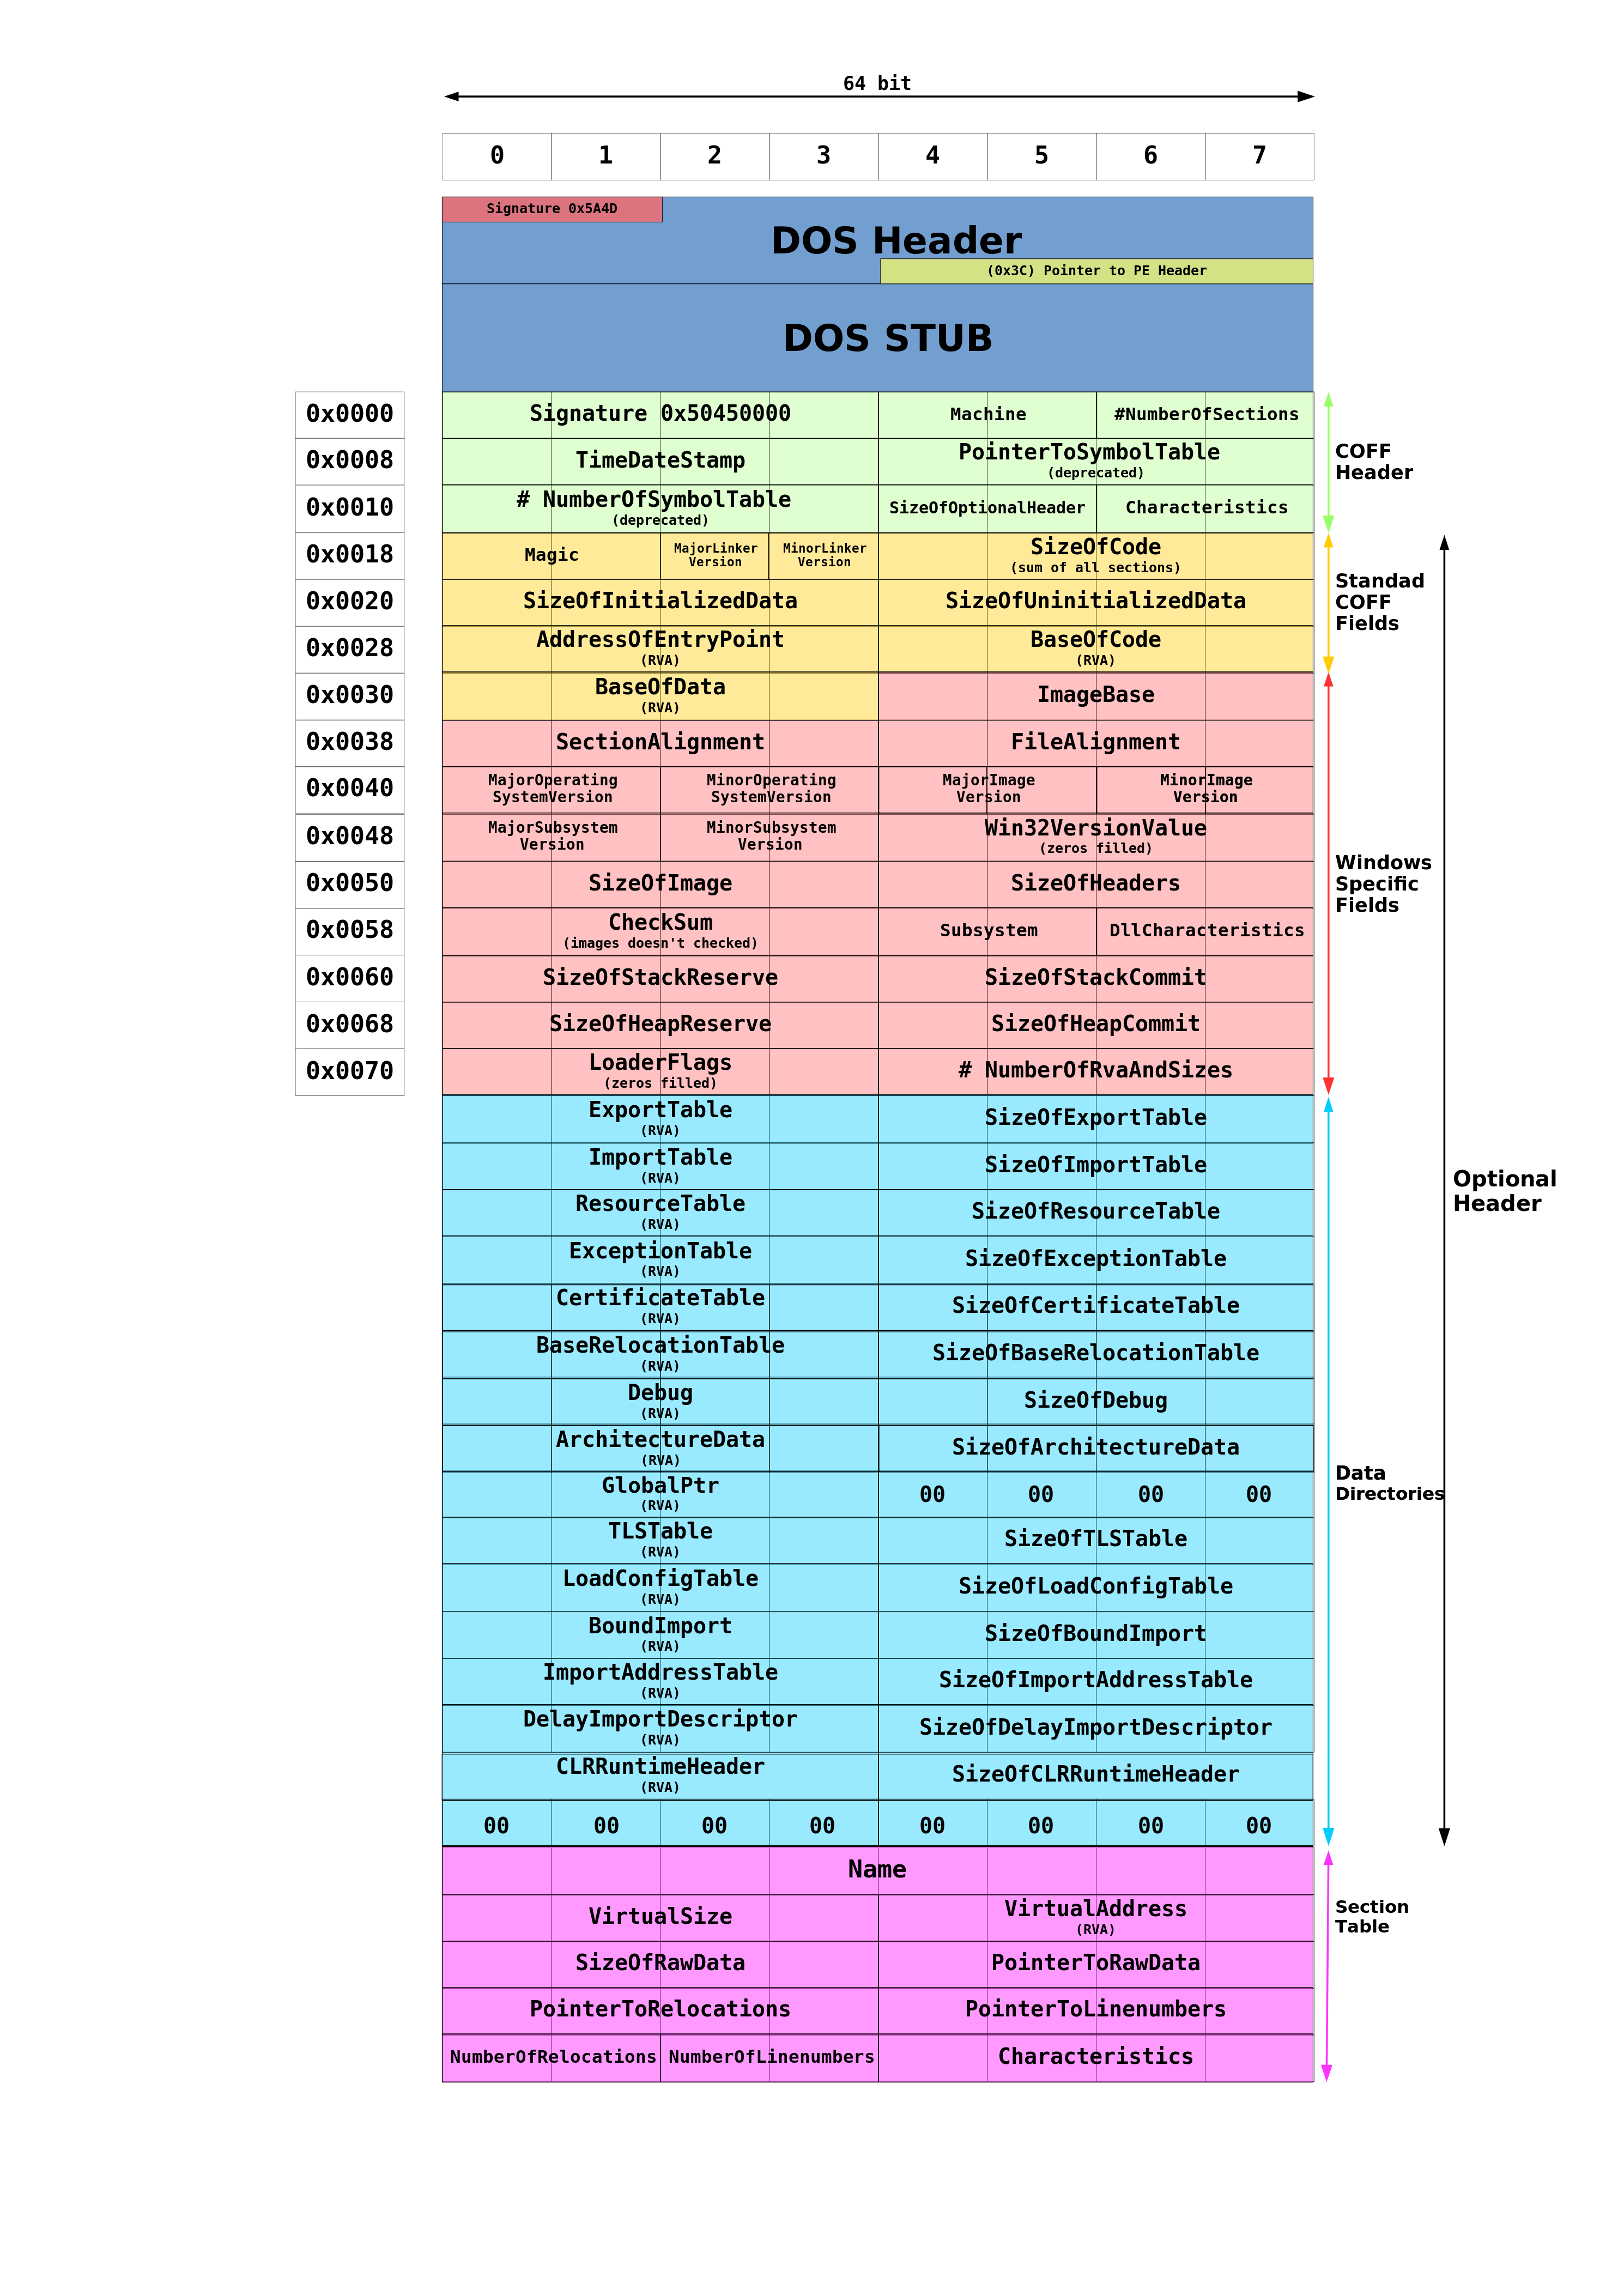
\includegraphics[width=1.0\textwidth]{Portable_Executable_32_bit.png}
\caption{Structure of a Portable Executable 32 bit \cite{wikipefile}}
\label{fig:pe32bit}
\end{figure}

PE sections contain code and initialized data that the Windows loader is to map into executable or readable/writeable memory pages, individually, as well as imports, exports, and resources defined by the file. Each section contains a header that specifies the size and address. An import address table instructs the loader which functions to import statically. A resources section may contain resources required for user interfaces such as: cursors, fonts, bitmaps, icons, menus, etc. A basic PE file would commonly contain a .text code section and one or more data sections (.data, .rdata or .bss). Relocation tables are typically stored in a .reloc section, used by the Windows loader to reassign a base address from the executable’s preferred base. A .tls section contains special thread local storage (TLS) structure for storing thread-specific local variables. Section names are random from the perspective of the Windows loader, but specific names have been adopted by precedent and are overwhelmingly common.

\section{Machine Learning}

\subsection{Introduction}
\label{ssec:machine-learning-intro}

In recent years, most of the productive research and advancements have come from the sub-discipline of Artificial Intelligence named Machine Learning. The principle of Machine Learning is straightforward; Machine Learning is a method by which computers find patterns in data and makes those patterns available to applications. The application can then gain insights on new data based on similarity to the identified patterns \cite{martin2016machine}.

\begin{figure}[htbp!] 
\centering    
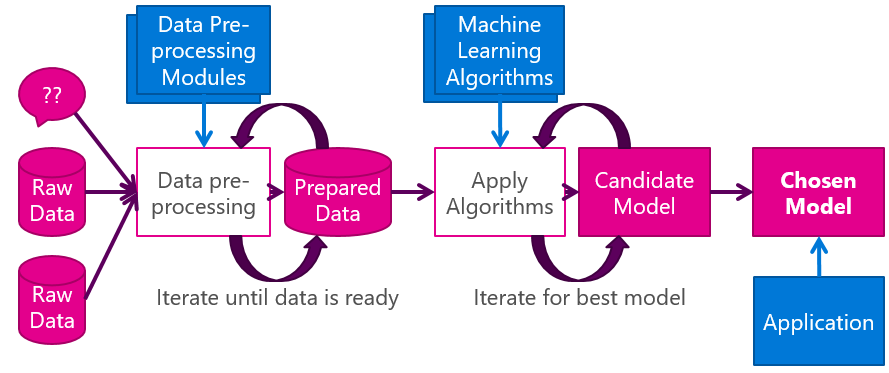
\includegraphics[width=1.0\textwidth]{MLProcess.png}
\caption{Machine Learning process \cite{martin2016machine}}
\label{fig:ml-process}
\end{figure}

It is worth going through the general workflow (Figure \ref{fig:ml-process}) of the machine learning process to have a deeper understanding:

\begin{itemize}
\item The primary goal of the process is to identify a model. The model is the main thing that applications can submit requests to gain insight on new data.
\item Before moving into Machine Learning experiments, we must identify the purpose and how to evaluate the result.
\item The process starts with preparing data. Prepared data is one or more data sets that have been preprocessed (formatted, cleaned and sampled) in readiness to apply Machine Learning algorithms. Preparing the data means that the data is in the best shape to draw scientific conclusions.
\item The next step is applying one or more Machine Learning algorithms intending to producing a Model, which is an iterative process and we may loop around testing various algorithms until we achieve a model that sufficiently reach the purpose.
\end{itemize}

Not all problems are candidates for a machine learning solution. The problem must be one that can be solved with data, and a sufficient quantity of relevant data must exist and be acquirable. As we shall see, many security problems fit this profile exceedingly well.

\subsection{Supervised Learning}
\label{ssec:supervised-learning}

Supervised learning algorithms make predictions based on a set of samples, e.g., historical stock prices can be used to try to guess at future prices. A supervised learning algorithm looks for patterns in labeled data. It can use any information that might be relevant, and each algorithm looks for different types of patterns. After the algorithm has detected the best pattern it can, it uses that pattern to make predictions for unlabeled data.

When the data are being used to predict a category, supervised learning is also called classification, e.g., assigning an image as a picture of either a cat or a dog. When there are only two choices, it is called two-class, binomial or binary classification. When there are more categories, this problem is known as multi-class classification.

\subsection{Feature Extraction}

As mentioned in section \ref{ssec:machine-learning-intro}, we should extract the attributes from the input data so that we can feed it into the algorithm. For example, in the image cases, data can be represented as an RGB value of each pixel.

Such attributes are referred to \textbf{features}, and the matrix is referred to as feature vector. The process of extracting data from the files is called feature extraction. The goal of feature extraction is to obtain a set of informative and non-redundant data. 

It is essential to understand that features should represent the necessary and relevant information about our dataset since we cannot make an accurate prediction without it. That is why feature extraction is often a non-obvious and domain-specific task, which requires a lot of testing and research.

Another critical requirement for a suitable feature set is non-redundancy. Having redundant features, i.e., elements that outline the same information, as well as irrelevant information attributes, that are strictly dependent on each other, can make the algorithm biased and, accordingly, provide an inaccurate result.

Furthermore, if the input data has too many features, it will take more training time. Hence, we may need to reduce the vector dimensions, which is known as the feature selection.

\subsection{Classification, Regression and Thresholding}

\textbf{Classification} is the task of approximating a mapping function ($f$) from input variables ($X$) to discrete output variables ($y$). The output variables are often called labels or categories. The mapping function predicts the class or group for a given observation. For example, an email can be classified as belonging to one of two categories: "spam" and "not spam".

\textbf{Regression} is the task of approximating a mapping function ($f$) from input variables ($X$) to a continuous output variable ($y$). An output variable is a real-value, such as an integer or floating point value. These are often quantities, such as amounts and sizes. For example, a house may be predicted to sell for a specific dollar value, perhaps in the range of \$100,000 to \$200,000.

Classification problems are different from regression problems. Classification is the task of predicting a discrete class label, and regression is the task of predicting a continuous quantity. However, there is some overlap between the algorithms for classification and regression.
For example, we can use the probability, which is returned from logistic regression, "as is" or convert it to a binary value. To map a logistic regression value to a binary category, we must define a \textbf{classification threshold} (also called the decision threshold). It is tempting to assume that the classification threshold should always be 0.5, but thresholds are dependent on the specific problems, and therefore values that we must tune.

\subsection{Ensemble, Bagging and Boosting}

When we try to predict the target variable using any machine learning method, the leading causes of difference in original and predicted values are noise, variance, and bias. The ensemble helps to reduce these two last factors.

An ensemble is just a collection of predictors which come together (e.g., mean of all predictions) to give a final prediction. The principal reason is that many different predictors trying to predict same target variable will perform a better job than any single one alone. Ensembling techniques are further classified into Bagging and Boosting.

Bagging is a simple ensembling technique in which we build many independent models and combine them using some model averaging methods (e.g., weighted average, majority vote or normal average). We typically use random sub-sample of data for each model, so that all the models are little different from each other. Each observation has the same probability to appear in all the models. Because this technique takes many uncorrelated predictors to make a final model, it reduces error by reducing variance. One example of bagging ensemble is Random Forest (which is mentioned in section \ref{ssec:random-forest}).

Boosting is an ensemble technique in which the models are not made sequentially. This technique applies the logic in which the following predictors learn from the mistakes of the previous ones. Accordingly, the observations have an unequal probability of appearing in subsequent models. The predictors can be chosen from a range of models like decision trees, regressors, classifiers, etc. Because new predictors are learning from mistakes committed by previous predictors, it takes fewer iterations to reach close to actual predictions. But we have to choose the stopping rules carefully, or it could lead to overfitting on training data. Gradient Boosting Decision Tree, in section \ref{ssec:gbdt}, is an example of boosting algorithm.

\section{Machine Learning Methods}

\subsection{Decision Tree}
\label{ssec:decision-tree}

As it assumes from the name, decision trees are data structures that have a structure of the tree. The training dataset is used for the creation of the tree, that is consequently used for making predictions on the test data. In this algorithm, the goal is to achieve the most accurate result with the least number of the decisions that must be made. We can use decision trees can for both classification and regression problems. There is an example in Table \ref{table:decision-tree}.

\begin{table}[h]
\caption{An example of decision tree}
\centering
\label{table:decision-tree}
\begin{tabular}{c l l c c c c}
\hline
Id & Name                       & Sex    & Age  & SibSp & Survived \\	
\hline
1  & Braund, Mr. Owen Harris    & male   & 22.0	& 1     & 0	\\
2  & Cumings, Mrs. John Bradley & female & 38.0	& 1     & 1	\\
3  & Heikkinen, Miss. Laina	    & female & 26.0	& 0     & 1 \\
...& ...                        & ...    & ...  & ...   & ... \\ 
\hline 
\end{tabular}
\end{table}

\begin{figure}[htbp!] 
\centering    
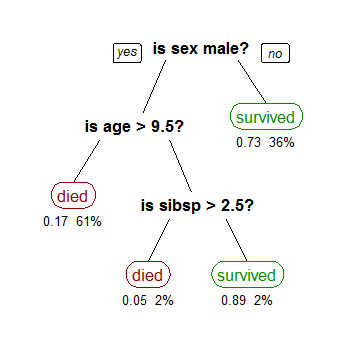
\includegraphics[width=0.5\textwidth]{decision_tree.png}
\caption{An example of decision tree \cite{wikidecisiontree}}
\label{fig:decision-tree}
\end{figure}

As you can see in Figure \ref{fig:decision-tree}, the model was trained based on the dataset and can now classify the passenger in Titanic is survived or not. The tree consists of the decision nodes and leaf nodes, and decision nodes may have several branches leading to leaf nodes. Leaf nodes represent the decisions or classifications. The first initial node is referred to as root node.

Decision tree method gained its popularity because of its simplicity. It can deal well with large datasets and can handle the noise in the datasets very well. Another advantage is that unlike other algorithms, such as SVM or KNN, decision trees operate in a white box, meaning that we can see how the outcome is obtained and which decisions led to it.

\subsection{Random Forest}
\label{ssec:random-forest}

Random Forest is one of the most common machine learning algorithms. It requires almost no data preparation and modeling but usually ends in inaccurate results. Random Forests are based on the decision trees described in the previous section \ref{ssec:decision-tree}. More specifically, Random Forests are the collections of decision trees, producing a better prediction accuracy. That is why it is called a forest – it is a set of decision trees.

The essential idea is to grow multiple decision trees based on the independent subsets of the dataset. At each node, \textit{n variables} out of the feature set are selected randomly, and the best split on these variables is found.


We can describe the algorithm as follows \cite{biau2012analysis}:

\begin{enumerate}
\item Multiple trees are built approximately on the two third of the training data randomly.
\item Several variables are randomly selected out of all the predictor variables. Then, the best split on these is used to split the node. By default, the amount of the selected variables is the square root of the total number of all predictors, and it is constant for all trees.
\item With the rest of the data, the misclassification rate is calculated. The total error rate is calculated as the overall out-of-bag error rate.
\item Each trained tree gives its classification result and the class that received the highest score is chosen as the result.
\end{enumerate}

Since we are using multiple decision trees, this algorithm removes the need for feature selection for removing unnecessary features – they will not be taken into account in any case. The only need for any feature selection with the random forest algorithms arises when there is a demand for dimensionality reduction. Moreover, the out-of-bag error rate, which was mentioned earlier can be considered the algorithm’s cross-validation method. This removes the need for tedious cross-validation measures, that would have to be taken otherwise \cite{mitchell1997machine}.

Random forests inherit many of the advantages of the decision trees algorithms. They are suitable for both regression and classification problems; they are easy to compute and quick to fit. They also regularly result in the better accuracy. However, unlike decision trees, it is not very easy to interpret the results. In decision trees, by examining the resulting tree, we can gain valuable information about which variables are relevant and how they affect the result. Random forests can also be described as a more firm algorithm than the decision trees since it is the combination of many decision trees, the random forest will remain stable \cite{louppe2014understanding}.

\subsection{Gradient Boosting Decision Trees}
\label{ssec:gbdt}

Gradient Boosting Decision Tree (GDBT) is an ensemble model of decision trees, which are trained in sequence \cite{friedman2001greedy}. 
In each iteration, GBDT learns the decision trees by fitting the negative gradients (also known as residual errors).
The main cost in GBDT lies in learning the decision trees, and the most time-consuming part of learning a decision tree is to find the best split points.
One of the most common algorithms to find split points is the pre-sorted algorithm \cite{mehta1996sliq, shafer1996sprint}, which lists all possible split points on the pre-sorted feature values. 
This algorithm is simple and can find the optimal split points.
However, it is wasteful in both training speed and memory consumption. Another famous algorithm is the histogram-based
algorithm \cite{ranka1998clouds, jin2003communication, li2008mcrank}. 
Instead of finding the split points on the sorted feature values, histogram-based algorithm buckets continuous feature values into discrete bins and uses these bins to construct feature histograms during training.

\bigskip
\begin{algorithm}[H]
 \KwData{$I$: training data, $d$: max depth}
 \KwData{$m$: feature dimension}
 $nodeSet \leftarrow \{0\} \triangleright$ tree nodes in current level \\
 $rowSet \leftarrow \{\{0, 1, 2, ...\}\} \triangleright$ data indices in tree nodes \\
 \For{$i = 1$ \KwTo $d$}{
  \For{$node$ \textbf{in} $nodeSet$}{
    $usedRows \leftarrow rowSet[node]$ \\
    \For{$k = 1$ \KwTo $m$}{
      $H \leftarrow$ new Histogram() \\
      $\triangleright$ Build histogram \\
      \For{$j$ \textbf{in} $usedRows$}{
        bin $\leftarrow$ I.f[k][j].bin \\
        H[bin].y $\leftarrow$ H[bin].y + I.y[j] \\
        H[bin].n $\leftarrow$ H[bin].n + 1
      }
    }
  }
  Update $rowSet$ and $nodeSet$ according to the best split points
 }
 \caption{Histogram-based Algorithm}
 \label{alg:histogram-based}
\end{algorithm}
\bigskip

As shown in Algorithm \ref{alg:histogram-based}, the histogram-based algorithm finds the best split points based on the feature histograms. 
It costs $O(\#data \times \#feature)$ for building histogram and $O(\#bin \times \#feature)$ for finding the split point. Since $\#bin$ is usually much smaller than $\#data$, histogram building will control the computational complexity. If we can reduce $\#data$ or $\#feature$, we will be able to speed up the training of GBDT extensively.

\subsection{Support Vector Machine}

Support Vector Machines (SVM) is another machine learning algorithm that is commonly used for classification problems. The main idea relies on finding such a hyperplane, that would separate the classes in the best way. The term "support vectors" refers to the points lying closest to the hyperplane, that would change the hyperplane position if removed. The distance between the support vector and the hyperplane is referred to as margin.

Intuitively, we know that the further from the hyperplane our groups lie, the more accurate predictions we can get. That is why, although multiple hyperplanes can be found, the goal of the SVM algorithm is to find such a hyperplane that would result in the maximum margins.

SVMs are usually able to produce good accuracy, particularly on clean datasets. 
Further, it is good at working with the high-dimensional datasets, also when the number of dimensions is higher than the number of the samples. 
Additionally, for large datasets with a lot of noise or overlapping classes, it can be more effective.
However, with more massive datasets training time can be extended \cite{jing2010view}.

\subsection{K-Nearest Neighbors}

The k-Nearest Neighbors algorithm (k-NN) is a non-parametric method used for classification and regression. 
The k-NN does not make any assumptions about the data structure, which makes it become a good solution in the real world where most of the data does not follow the typical theoretical assumptions. 
K-NN is also a lazy algorithm, which means there is no specific training phase or it is very insignificant. 
Also, lack of generalization means that k-NN keeps all the training data, i.e., the most the training data is required during the testing phase.

The algorithm is based on feature similarity. 
How closely out-of-sample features match the training set determines how k-NN classify a given data point.
The Euclidean Distance,  which is defined by the formula below, is the most used method for continuous variables in k-NN.

\begin{center}
$EuclideanDistance =  \sqrt{ \sum_{i=1}^{n}(q_i - p_i)^2 }$
\end{center}

The drawback of the k-NN algorithm is the lousy performance on the unevenly distributed datasets. 
Hence, if one class hugely overshadows the other ones, it is more likely to have more neighbors of that class due to their large number, and therefore, make incorrect predictions \cite{laaksonen1996classification}.

\subsection{Neural Networks}

\subsubsection{Overview}

The idea behind neural networks, i.e., having computational units that produce “intelligent” results only through interactions with each other, was inspired by the brain. 
For instance, the Neocognitron system, proposed by Kunihiko Fukushima in 1980, took inspiration from the mammalian visual system and laid the foundation for modern convolutional networks \cite{goodfellow2016deep}. 
Hence, the artificial neurons in these networks mimic the structure of biological ones. 

The very first artificial model of the biological neuron is in fact perceptron, introduced by Frank Rosenblatt in 1958 \cite{rosenblatt1958perceptron}. 
Perceptron is an algorithm for supervised learning in machine learning. Perceptron, in essence, is a simple function that turns inputs (usually a real-valued vector) into one binary output.

\begin{figure}[htbp!] 
\centering    
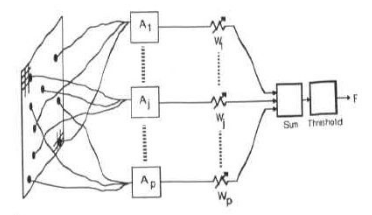
\includegraphics[width=0.5\textwidth]{perceptron.png}
\caption{Basic structure of a perceptron \cite{minsky1969perceptron}}
\label{fig:perceptron}
\end{figure}

Following Figure \ref{fig:perceptron}, we can see the perceptron receives \textit{p} inputs, $A_1$, $A_2$, ..., $A_p$ (or $x_1$, $x_2$, ..., $x_p$, depending on the source. 
The inputs are then respectively weighted by $w_1$, $w_2$, ..., $w_p$, which are real numbers indicating the importance of each of the input values. The output \textit{F} will then be calculated using the sum of those weighted inputs. 
Additionally, because the output is a binary value, a threshold is used to achieve the desired result. To be more specific, a perceptron is written as follows:

\begin{center}
$F = \begin{cases}
1 & if \sum_{i}^{p} A_i w_i \geq Threshold \\
0 & if \sum_{i}^{p} A_i w_i < Threshold
\end{cases}$
\end{center}

Consequently, the output of a perceptron is controlled by two things: the weights $w_1$, $w_2$, ..., $w_p$ and the Threshold. 
In modern neuron networks, however, the equation changed a bit by bringing the Threshold to the other side of the inequalities. 
The additive inverse of Threshold is then known as Bias, and the perception will be rewritten as:

\begin{center}
$F = \begin{cases}
1 & if \sum_{i}^{p} A_i w_i + Bias \geq 0 \\
0 & if \sum_{i}^{p} A_i w_i + Bias < 0
\end{cases}$
\end{center}

\subsubsection{Activation function}

Perceptron is the precursor to modern artificial neurons. Instead of returning only a binary output, an artificial neuron now produces values that are anywhere in the range [0,1]. 
The reason is to help in the learning process of a network. Neural networks can learn, i.e., finding the appropriate weights and biases given sufficient input data. 
The learning process, however, needs to be progressive, which means weights and biases get increasingly close to the "good" values. 
Having a binary output for each of the neurons makes it hard for this process to be done. 
For training a neural network, we use an error function to see how far or close the network is to the optimal results.
Because of the binary output of perception, a small change in the network's parameters can lead to a stark difference for the output, making it hard to tune the parameters to achieve a good result. 
Therefore, modifications must be made to the original perceptron model. 
Instead of using 0 as the threshold at which signals are allowed to be fired, we can use an activation function to map the output to the range we need appropriately.

\begin{figure}[htbp!] 
\centering    

\includegraphics[width=0.7\textwidth]{artificial_neuron.png}
\caption{Structure of an artificial neuron \cite{wikian}}
\label{fig:artificial-neuron}
\end{figure}

The activation function takes as input the weighted sum of the input values fed to the perceptron and returns a value in the range [0,1]. 
Historically, the Sigmoid function was used for this purpose as it can squash the sum to the desired range \cite{li2015cs231n}. 
Modern networks, however, use different functions as well, such as hyperbolic tan function (tanh) or rectified linear unit (ReLU), to achieve better performance \cite{li2015cs231n}.

\subsubsection{Feedforward and Backpropagation}

Two operations are particularly important in neural networks: Feedforward and Backpropagation.

Feedforward is used in both the training and testing stage of a network. 
The task we need to do in feedforward is straightforward: Passing output of a layer as the input of the next layer.
Since all we are doing is unidirectionally putting values through the network from the input layer to the output layer, the operation is called feedforward. 

Backpropagation is generally used in the training stage to help neural networks learn their parameters, and it is considered an optimization. 
Different from feedforward, the job of this operation is to propagate error of the output values back to the network to update the network parameters. 
Backpropagation works by first do the normal feedforward operation on the network with the given input. 
After the output is obtained, we compare the output to the desired output, using a loss function to generate an error term for each of the neuron in the output layer. 
The error values are then propagated backward from the output layer until every neuron receive their respective error term. 
The error terms will be used to calculate the gradient, with which we can update the weights of the network to minimize the loss function as the process repeats. 
To find the most fitting parameters, gradient descend algorithm is usually applied.

\section{Classification Metrics}

In this section, we review how to use several common metrics that are used to evaluate predictions for classification problems.

\subsection{Logarithmic Loss}

Logarithmic loss, or log-loss for short, is a performance metric for evaluating the predictions of probabilities of membership to a given class.

Log-loss takes into account the uncertainty of your prediction based on how much it varies from the actual label, which gives us a more nuanced view of the performance of our model.
In binary classification, with $y$ is a binary indicator (0 or 1) of whether class label $c $is the correct classification and $p$ is the model predicted probability, the formula equals:

\bigskip
\begin{center}
    $LogLoss = -(y\log(p) + (1 - y)\log(1 - p))$
\end{center}
\bigskip

The scalar probability between 0 and 1 can be seen as a measure of confidence for a prediction by an algorithm.
Smaller log-loss is better with 0 representing a perfect log-loss.

\subsection{Confusion Matrix}
\label{ssec:confusion_matrix}

\begin{figure}[H]
    \centering    
    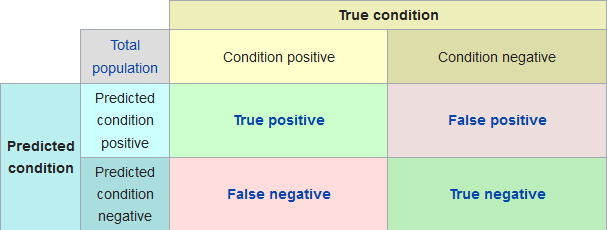
\includegraphics[width=0.7\textwidth]{confusion_matrix.png}
    \caption{Confusion matrix \cite{wiki_confusion_matrix}}
    \label{fig:confusion_matrix}
\end{figure}

A clean and unambiguous way to show the prediction results of a classifier is to use a confusion matrix (also called a contingency table).
For a binary classification problem, the table has two rows and two columns (which is shown in Figure \ref{fig:confusion_matrix}). 
Across the top is the actual class labels and down the side are the predicted class labels. 
Each cell carries the number of predictions made by the classifier that fall into that cell.

\begin{figure}[H]
    \centering    
    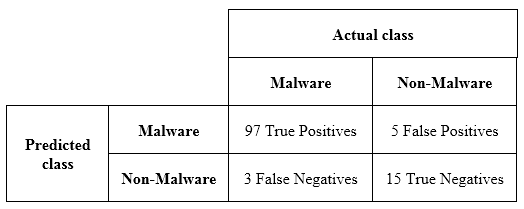
\includegraphics[width=0.7\textwidth]{confusion_matrix_example.png}
    \caption{An example of confusion matrix}
    \label{fig:confusion_matrix_example}
\end{figure}

Figure \ref{fig:confusion_matrix_example} is an example of binary classification in malware detection. 
Some of the input files are malware, and our test correctly says they are positive. 
They are called true positives (TP). 
In contrast, some are malware, but the test incorrectly claims they are not. 
They are called false negatives (FN). 
Some are clean files, and the test says they are not malware – true negatives (TN). 
Finally, there might be clean files have a positive test result – false positives (FP).

There are many derived ratios from confusion matrix, and the most common ones are listed below:

\begin{itemize}
    \item True Positive Rate (TPR), eqv. with hit rate, recall: $TPR = TP/P = TP/(TP + FN)$
    \item True Negative Rate (TNR): $SPC = TN/N = TN/(TP + FN)$
    \item Precision or Positive Predictive Value (PPV): $PPV = TP/(TP + FP)$
    \item Negative Predictive Value (NPV): $NPV = TN/(TN + FN)$
    \item Fall-out or False Positive Rate (FPR): $FPR = FP/N = FP/(TP + FN) = 1 - TNR$
    \item False Discovery Rate (FDR): $FDR = FN/(FN + TP) = 1 - PPV$
    \item Miss Rate or False Negative Rate (FNR): $FNR = FN/(FN + TP) = 1 - TPR$
\end{itemize}

\subsection{Overall Accuracy}

Overall accuracy is the number of correct predictions made as a ratio of all predictions made.

\begin{center}
    ${Accuracy} =  \cfrac{True\ positive + True\ negative}{Condition\ positive + Condition\ negative}$
\end{center}

Overall Accuracy essentially tells us out of all of the reference sites what proportion were mapped correctly. 
The overall accuracy is usually expressed as a percent, with 100\% accuracy being a perfect classification where all reference site were classified correctly. 
Overall accuracy is the easiest to calculate and understand but ultimately only provides the map user and producer with necessary accuracy information.

This is the most common evaluation metric for classification problems, it is also the most misused. 
It is only suitable when there is an equal number of observations in each class (which is rarely the case) and that all predictions and prediction errors are equally important (which is often not the case).

\subsection{Precision and Recall}

Precision can be thought of as a measure of a classifiers exactness. Precision attempts to answer the question "What proportion of positive identifications was actually correct?". A low precision can also indicate a large number of False Positives.

\begin{center}
    ${Precision} =  \cfrac{True\ positive}{True\ positive + False\ positive}$
\end{center}

Recall is the number of True Positives divided by the number of True Positives and the number of False Negatives. Computing in another way is the number of positive predictions divided by the number of positive class values in the test data. Recall attempts to answer "What proportion of actual positives was identified correctly?". It is also called Sensitivity or the True Positive Rate.

\begin{center}
    ${Recall} =  \cfrac{\sum True\ positive}{\sum Condition\ positive}$
\end{center}

\subsection{Area Under ROC curve}
\label{ssec:auroc}

Area Under the Receiver Operating Characteristic curve, AUROC or AUC for short, is a performance metric for binary classification problems. The AUROC has several equivalent interpretations:

\begin{itemize}
\item The expectation that a uniformly drawn random positive is ranked before a uniformly drawn random negative.
\item The expected proportion of positives ranked before a uniformly drawn random negative.
\item The expected true positive rate if the ranking is split just before a uniformly drawn random negative.
\item  The expected proportion of negatives ranked after a uniformly drawn random positive.
\item  The expected false positive rate if the ranking is split just after a uniformly drawn random positive.
\end{itemize}

An area of $1.0$ represents a model that made all predictions perfectly. A rough guide for classifying the accuracy of a classification test is the typical academic point system: 

\begin{itemize}
\item 0.9 - 1.0 = Excellent
\item 0.8 - 0.9 = Good
\item 0.7 - 0.8 = Fair
\item 0.6 - 0.7 = Poor
\item 0.5 - 0.6 = Fail
\end{itemize}

\subsubsection{Compute the AUROC}

Assume we have a binary classifier such as logistic regression. First, we compute two metrics from the confusion matrix (their formula are mentioned in section \ref{ssec:confusion_matrix}), which will be later combined into one:

\begin{enumerate}
    \item \textbf{True positive rate (TPR).} Intuitively this metric agrees to the proportion of positive data points that are correctly considered as positive, with respect to all positive data points. In other words, the higher TPR, the fewer positive data points we will miss.
    \item \textbf{False positive rate (FPR).} This metric corresponds to the proportion of negative data points that are mistakenly considered as positive, concerning all negative data points. In other words, the higher FPR, the more negative data points will be misclassified.
\end{enumerate}

\begin{figure}[H]
    \centering    
    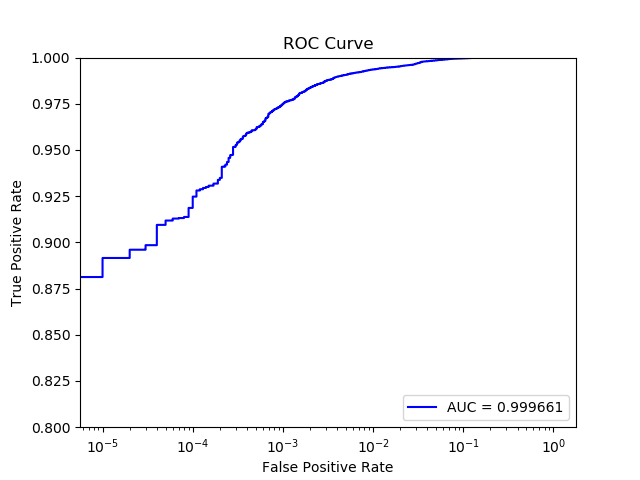
\includegraphics[width=0.8\textwidth]{roc_curve.png}
    \caption{An example of Receiver Operating Characteristic curve}
    \label{fig:auroc}
\end{figure}

Then, we combine the FPR and the TPR into one single metric by computing the two former metrics with many different threshold (for example, 0.00, $10^-5$, $10^-4$, $10^-3$, ..., 1.00, as shown as in Figure \ref{fig:auroc}) for the logistic regression, then plot them on a single graph, with the FPR values on the x-axis and the TPR values on the y-axis. The resulting curve is called  Receiver Operating Characteristic curve, and the metric we consider is the area under this curve.

\section{LightGBM - A Gradient Boosting Framework}

LightGBM, which means Light Gradient Boosting Machine, is a gradient boosting framework that uses tree-based learning algorithm \cite{ke2017lightgbm}. This framework is obtaining an extreme reputation due to its following advantages:

\begin{itemize}
\item Faster training speed and higher efficiency
\item Lower-memory usage
\item Better accuracy
\item Parallel and GPU learning supported
\item Capable of handling the large-scale data
\end{itemize}

The framework uses two following techniques to solve problems when the feature dimension is high, and data size is considerable: Gradient-based One-Side Sampling and Exclusive Feature Bundling.

\subsection{Gradient-based One-Side Sampling}

Base on the notice that, while there is no weight for data instance in the gradient-boosting decision tree, data instances with different gradients play different roles in the computation of information gain. 
In particular, according to the definition of information gain, instances with larger gradients (i.e., under-trained instances) will contribute more to the information gain.
Since, when subsampling the data instances, to retain the accuracy of information gain estimation, LightGBM tends to keep instances with large gradients (e.g., larger than a pre-defined threshold, or among the top percentiles), and only randomly drops instances with small gradients.
They proved that such a treatment could lead to a more accurate gain estimation than uniformly random sampling, with the same target sampling rate, especially when the value of information gain has a vast range.

\subsection{Exclusive Feature Bundling}

Regularly in real applications, although there are a large number of features, the feature space is quite sparse, which provides the LightGBM a possibility of using a nearly lossless approach to reduce the number of active features.
In fact, in a sparse feature space, many features are almost exclusive, i.e., they rarely take nonzero values together, e.g., the one-hot encoding features, therefore, the framework could safely bundle such unique features.
LightGBM uses an efficient algorithm named Exclusive Feature Bundling, which is a greedy algorithm with a constant approximation ratio.
Specifically, they reduce the optimal bundling problem to a graph coloring problem by taking features as vertices and add edges for every two features if they are not together exclusive.

\section{Open Neural Network Exchange (ONNX)}
\label{sec:onnx}
 
Facebook and Microsoft introduced Open Neural Network Exchange (ONNX) format, a standard for representing deep learning models that enables models to be transferred between frameworks. 
ONNX is an open source format that empowers AI developers to choose the right tools as their project evolves.
 
At a high level, ONNX is designed to allow framework interoperability. There are many excellent machine learning frameworks, ones of them make use of static graphs ((such as CNTK, Caffe2, Theano, and TensorFlow), while others use dynamic graphs (such as PyTorch and Chainer).
The graph serves as an Intermediate Representation (IR) that captures the specific intent of the developer's source code and is conducive for optimization and translation to run on particular devices (CPU, GPU, FPGA, etc.).
By providing a common Intermediate Representation of the computation graph, ONNX helps developers choose the right framework for their task, allows authors to focus on innovative enhancements, and enables hardware vendors to streamline optimizations for their platforms.
 
\section{Windows ML}
 
Windows ML is a platform that evaluates trained machine learning models on Windows 10 devices, allowing developers to use machine learning within their Windows applications. 
Some highlights of Windows ML include:
 
\begin{itemize}
\item Hardware acceleration: On DirectX12 capable devices, Windows ML accelerates the evaluation of deep learning models using the GPU. Additionally, CPU optimizations enable high-performance evaluation of both classical machine learning and deep learning algorithms.
\item Local evaluation: Windows ML evaluates on local hardware, removing concerns of connectivity, bandwidth, and data privacy. The local evaluation also enables low latency and high performance for quick evaluation results.
\item Image processing: For computer vision scenarios, Windows ML simplifies and optimizes the use of the image, video, and camera data by handling frame pre-processing and providing camera pipeline setup for model input.
\end{itemize}
 
To use Windows ML, the developers need a pre-trained machine learning model in the Open Neural Network Exchange (ONNX) format, that is mentioned in section \ref{sec:onnx}. 
Windows ML supports the v1.0 release of the ONNX format, which allows developers to use models produced by different frameworks.

\chapter{Proposed Method}
\graphicspath{{Chapter4/Figs/}}

\begin{chapabstract}
This chapter describes how to extract features from Portable Executable files, the Gradient Boosting Decision Trees model we used, and the reasoning behind.
\end{chapabstract}

\section{Feature Extraction}
\label{sec:feature-extraction}

Inspired by Hyrum S. Anderson and Phil Roth from Endgame, Inc. \cite{anderson2018ember}, we extracted each PE file into eight feature groups which can be classified into two types: format-agnostic features and parsed features.

\subsection{Format-agnostic Features}

We use three groups of features to model the contents of input files in a file-format agnostic way, meaning that it has no dependencies on its format. By providing the simple statistical summaries rather than a listing of raw features, e.g., all bytes or all strings, we decrease privacy concerns and are easy to request or publish the dataset.

\subsubsection{Byte-Entropy Histogram}

Based on the work published by Joshua Saxe and Konstantin Berlin \cite{saxe2015deep}, they show that, in practice, the effect of representing byte values in the entropy context in which they occur separates byte values that arise in the context of, for example, x86 instruction data from, for example, byte values occurring in compressed data.

To compute the byte-entropy histogram, we slide a 2048-length window over all the input bytes with a step size of 1024 bytes. Use a simple trick to calculate the entropy $H$ faster, i.e., reducing the information by half, and pairing it with each byte within the window. Then, we compute a two-dimensional histogram with $16 \times 16$ bins that quantize entropy and the byte value. Finally, we concatenate each row vector in the matrix and normalize the final 256-value vector.

\subsubsection{Byte Histogram}

The byte histogram is a 256-value vector which represents the distribution of each byte value within the file.

\subsubsection{String Information}

The final format-agnostic group of features is string information. These features are derived from the printable sequences of characters in the range \verb|0x20| to \verb|0x7f|, that have at least five characters long. We use the number of strings, the average length of these strings, the amounts of lines  that may sequentially indicate a path (begin with \verb|C:\|), an URL(start with \verb|http://| or \verb|https://|), a registry key (the occurrences of \verb|HKEY_|) and a bundled executable (the short string \verb|MZ|). Also, we use a histogram of the printable characters within these strings.

\subsection{Parsed Features}

In addition to using three format-agnostic groups of features, we extract five other groups from parsing the Portable Executable file by using LIEF - Library to Instrument Executable Formats \cite{lief}.

\subsubsection{General Information}

The set of features includes the file size and necessary information collected from the PE header: the virtual size of the file, the number of imported and exported functions, the number of symbols, whether the data has a debug section, thread local storage, resources, relocations, or a signature.

\subsubsection{Header Information}

We use the information from the Common Object File Format (COFF) header including the timestamp in the header, the target machine and a list of image characteristics. And from the optional header, we use the target subsystem, DLL  characteristics,  the file magic as a string, major and minor image versions, linker versions, system versions and subsystem versions, and the code size, header size and commit size. We use hashing trick with 10 bins for string features \cite{weinberger2009feature}.

\subsubsection{Imported Functions}
\label{sssec:imported}

Parsing the import address table gives us a report about the imported functions by libraries. We use the set of unique libraries with 128-bin hashing trick. Similarly, we apply the 512-bin hashing trick to capture individual functions, by representing
it in string format \verb|library:function|, for example, \verb|kernel32.dll:CreateFileMappingA|.

\subsubsection{Exported Functions}

Similar to extracting imported functions, we summarize a list of the exported functions into a 128-value vector by hashing.

\subsubsection{Section Information}

Properties of each section are used: the name, size, entropy, virtual size, and a list of strings representing section characteristics. We still use the hashing trick on \verb|(section name, value)| pairs to create 50-value vectors containing section size, section entropy, virtual size, and information about entry point characteristics.

\section{Classification}
 
For classification, in this study, we use the Gradient Boosting Decision Trees algorithm with 400 iterations and 64 leaves in one tree. We configure that there must be at least 200 samples in one child, and set learning rate at 5 percent. We elaborate on the reasoning behind these choices below.

Firstly, the massive number of features causes scalability issues for many machine learning algorithms.  For example,  non-linear  SVM  kernels require $O(N^2)$ multiplication during each iteration, and k-Nearest Neighbors (k-NN) requires significant computation and storage of all label samples during prediction. Accordingly, we target to use neural networks and ensemble decision trees, which are scalable alternatives.

Secondly, our resources, primarily financial support, are lacking. But the cost for training neural networks is extremely computationally expensive. We tried with some complex models, and these take many hours and require costly more GPUs for speeding. Also, neural networks are the black-box that not much can be gleaned from and required much experience to optimize.

Besides, another scalable alternative, tree ensemble algorithms handle very well high dimensional feature spaces as well as a large number of training examples. The two most popular algorithms are Random Forests and Gradient Boosting Decision Trees (GDBT). GBDT training usually takes longer because trees are built sequentially. However, benchmark results have shown GBDT are better learners than Random Forests.

In practice, in our experiments, Gradient Boosting Decision Trees algorithm always takes less training time in comparing to neural networks with the same hardwares.

\chapter{Thực Nghiệm và Đánh Giá}
\graphicspath{{Chapter5/Figs/}}

\begin{chapabstract}
Firstly, we introduce the dataset used for training and evaluating in our experiments. We also present the evaluation metrics and explain the reason for choosing those criteria. Then, the experiment results are shown in comparing to other proposed models. Finally, we present how to set up the environments for experiments.
\end{chapabstract}

\section{Tập dữ liệu}
\label{sec:dataset}

Trong thử nghiệm của chúng tôi, chúng tôi sử dụng 600.000 mẫu đào tạo được dán nhãn và 200.000 mẫu thử nghiệm từ tập dữ liệu Endgame Malware BEnchmark for Research (EMBER) \cite{anderson2018ember}.

\begin{figure}[H] 
\centering
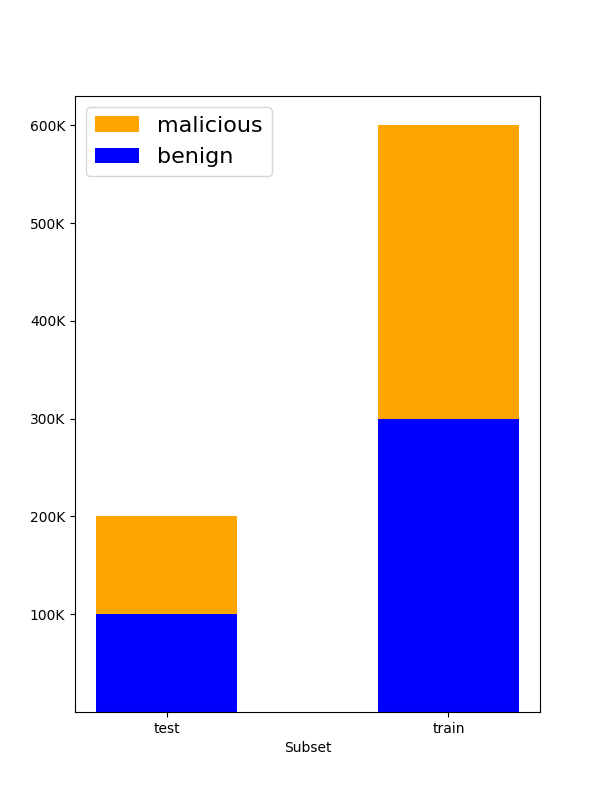
\includegraphics[width=0.5\textwidth]{dataset.png}
\caption{Phân phối mẫu trong tập dữ liệu.}
\label{fig:ember}
\end{figure}
 
Tập dữ liệu EMBER là tập dữ liệu công khai lớn để phát hiện phần mềm độc hại, nó bao gồm các tệp lành tính và có tỷ lệ lý tưởng các tệp độc hại và lành tính cho các tác vụ học máy. Điều này sẽ giải quyết vấn đề chung về độ chính xác dự đoán, cụ thể là vấn đề gây hiểu lầm khi dữ liệu bị mất cân bằng.

\section{Tiêu chí Đánh giá}

Như đã thảo luận trong phần \ref{sec:objectives}, mục tiêu của nghiên cứu là tìm ra phương pháp phát hiện phần mềm độc hại dựa trên học máy hoạt động ở tỷ lệ dương giả thấp trong khi cố gắng đạt được tỷ lệ phát hiện cao.

\subsection{Tỷ lệ Báo động sai}

Sai tích cự (False positive), hoặc báo động sai, xảy ra khi một mô hình sai lầm gán một nhãn độc hại cho một tập tin lành tính. 
Chúng tôi có tập trung làm cho tỷ lệ dương tính giả càng thấp càng tốt, đó là việc không điển hình trong ứng dụng học máy. 
Điều quan trọng là bởi vì ngay cả một báo động giả trong một nghìn tập tin lành tính có thể tạo ra hậu quả nghiêm trọng cho người dùng. 
Vấn đề này là phức tạp bởi thực tế là có rất nhiều tập tin sạch trên thế giới, chúng tiếp tục xuất hiện, và rất khó khăn để thu thập các tập tin này. Chúng tôi đánh giá phương pháp của chúng tôi với hai giá trị báo động giả, cụ thể: ở mức dưới 0,1\% và ở mức dưới 1\%.

\begin{center}
    ${False\ alarm\ rate} =  \cfrac{\sum False\ positive}{\sum Condition\ negative}$
\end{center}

\subsection{Tỷ lệ Phát hiện}

Tỷ lệ phát hiện, (tương đương với recall hoặc true positive rate), đo tỷ lệ các chương trình độc hại được phát hiện trong các tệp phần mềm độc hại được sử dụng để thử nghiệm. Với tỉ lệ cao hơn, ít trường hợp phần mềm độc hại trong thực tế không bị phát hiện. Nói cách khác, tỷ lệ phát hiện cho thấy tiềm năng của các tệp nhị phân độc hại mới sẽ được phát hiện.

\begin{center}
    ${Detection\ rate} =  \cfrac{\sum True\ positive}{\sum Condition\ positive}$
\end{center}

\subsection{Diện tích dưới đường cong ROC}

Như đã giới thiệu trong phần \ref{ssec:auroc}, phần Diện tích dưới đường cong ROC (Area Under the ROC curve, viết tắt là AUROC hoặc AUC) cung cấp thước đo tổng thể về hiệu suất trên tất cả các ngưỡng phân loại có thể có.
AUC là quy mô bất biến và đo lường dự đoán được xếp hạng tốt như thế nào, chứ không phải là giá trị tuyệt đối của chúng.
Bên cạnh đó, AUC là bất biến với ngưỡng phân loại, để nó có thể đo lường chất lượng của các dự đoán không phụ thuộc vào ngưỡng nào được chọn.
Một mô hình có dự đoán là 100\% sai có AUC là 0,0, và có một dự đoán là 100\% đúng có AUC là 1,0.

Hệ thống điểm học thuật điển hình để phân loại độ chính xác của bài kiểm tra phân loại như sau:

\begin{itemize}
\item 0.9 - 1.0 = Excellent
\item 0.8 - 0.9 = Good
\item 0.7 - 0.8 = Fair
\item 0.6 - 0.7 = Poor
\item 0.5 - 0.6 = Fail
\end{itemize}

\section{Kết quả Thực nghiệm}

Phương pháp phát hiện phần mềm độc hại dựa trên GBDT được đề xuất được triển khai với LightGBM framework \cite{ke2017lightgbm}, và các vectơ đặc trưng đầu vào có kích thước 1711. Tất cả các thử nghiệm của chúng tôi đều chạy trên một máy tính ảo hóa có 24 vCPUs và bộ nhớ 32 GB. Sử dụng lập trình song song, mất khoảng 10 phút để vector hóa các tính năng thô và khoảng 5 phút để đào tạo mô hình. Đường cong ROC của mô hình cuối cùng được thể hiện trong hình \ref{fig:roc_curve_with_highlights} và phân phối điểm số cho các mẫu thử được thể hiện trong hình \ref{fig:score_dist}.

\begin{figure}[H]
\centering
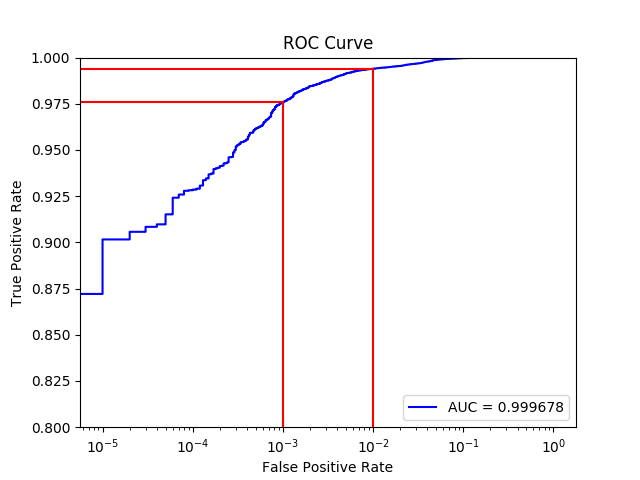
\includegraphics[width=\textwidth]{roc_curve_with_highlights.png}
\caption{The ROC curve of proposed model}
\label{fig:roc_curve_with_highlights}
\end{figure}

\begin{figure}[h] 
\centering
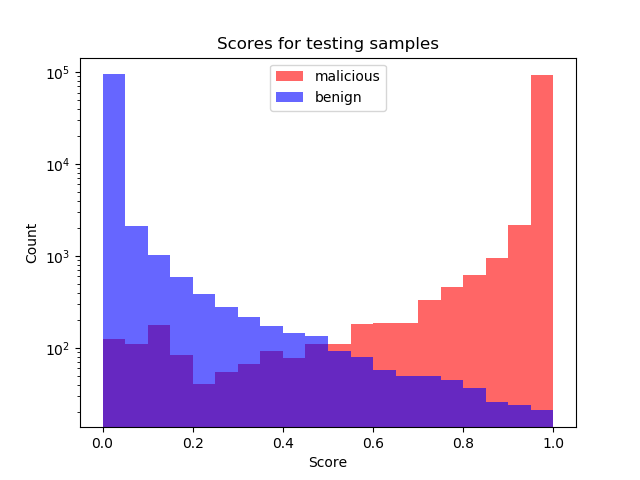
\includegraphics[width=\textwidth]{score_dist.png}
\caption{The distribution of scores for testing samples}
\label{fig:score_dist}
\end{figure}

Diện tích dưới đường cong ROC đạt mức $0.999678$. Với threshold $0.828987$, điểm kết quả của mô hình khi ít hơn $0.1\%$ tỉ lệ báo động sai có tỉ lệ phát hiện $97.5720\%$. Và với mức tỉ lệ báo động sai $1\%$, mô hình đạt tỉ lệ phát hiện $99.3940\%$ với threshold là $0.307897$. 

Mô hình cơ sở của EMBER chỉ có diện tích dưới đường cong ROC là $0.99911$, kết quả với mức $0.1\%$ FPR là $92.99\%$ TPR, và mức $1\%$ FPR, là $98.2\%$ TPR. Mô hình của chúng tôi có hiệu suất tốt hơn do điều chỉnh siêu tham số và cũng mất ít thời gian hơn cho việc đào tạo do giảm số lượng các đặc trưng.Rõ ràng, mô hình có hiệu suất tốt hơn so với mô hình MalConv được đào tạo trên các tệp nhị phân thô \cite{anderson2018ember}, nó có ROC AUC là $0.99821$, tương ứng với $92.2\%$ TPR ở mức báo động sai dưới 0.1\%, và 97.3\% TPR ở mức dưới 1\% FPR. Bảng \ref{table:training-time} và bảng \ref{table:results}hiển thị thời gian đào tạo và kết quả đánh giá của mô hình đề xuất của chúng tôi so với mô hình MalConv và mô hình cơ sở của EMBER.

\begin{table}[H]
\caption{Thời gian đào tạo của mô hình được đề xuất của chúng tôi so với mô hình MalConv và mô hình cơ sở của EMBER}
\centering
\label{table:training-time}
\begin{tabular}{l l l l}
\hline
Model & Input &  Specifications & Training time \\
\hline
MalConv & Raw binaries & \begin{tabular}[c]{@{}l@{}} 2 NVDIA TITAN X \\ (Pascal) GPUs \end{tabular}  & \begin{tabular}[c]{@{}l@{}}10 days\\ (25 hours/epoch)\end{tabular}  \\
EMBER & 2351-value vectors & \begin{tabular}[c]{@{}l@{}} 8 vCPUs \\ (2015 MacBook Pro i7)\end{tabular}  & 20 hours \\ 
Our model & \textbf{1711}-value vectors & \begin{tabular}[c]{@{}l@{}} 24 vCPUs \\ (Google Compute Engine) \end{tabular}  & \textbf{5 minutes }\\ 
\hline 
\end{tabular}
\end{table}

\begin{table}[H]
\caption{Kết quả đánh giá của mô hình được đề xuất của chúng tôi so với mô hình MalConv và mô hình cơ sở của EMBER}
\centering
\label{table:results}
\begin{tabular}{l c c c}
\hline
Model                      & \begin{tabular}[c]{@{}c@{}}False Alarm Rate\\ (FPR)\end{tabular} & \begin{tabular}[c]{@{}c@{}}Detection Rate\\ (TPR)\end{tabular} & \begin{tabular}[c]{@{}c@{}}Area Under\\ the ROC curve (AUC)\end{tabular} \\

\hline
\multirow{2}{*}{MalConv}   & 0.1 \%                 & 92.200 \%            & \multirow{2}{*}{0.998210}                                                 \\
                           & 1.0 \%                 & 97.300 \%            &                                                                           \\
\multirow{2}{*}{EMBER}     & 0.1 \%                 & 92.990 \%            & \multirow{2}{*}{0.999110}                                                 \\
                           & 1.0 \%                 & 98.200 \%            &                                                                           \\
\multirow{2}{*}{Our model} & 0.1 \%                 & 97.572 \%            & \multirow{2}{*}{0.999678}                                                 \\
                           & 1.0 \%                 & 99.394 \%            &                                                                          
\\
\hline 
\end{tabular}
\end{table}

\section{Hướng dẫn cài đặt môi trường} 
\label{sec:research-env}

We mainly use the cross-platform tools in research and development for easily switching between operating systems. We use a Windows 10 Pro virtual machine for static malware analysis, an Ubuntu 16.04 LTS cloud instance for training and testing machine learning models, and use PyCharm Professional as mainly Integrated development environment (IDE).

\subsection{Windows environment for static analysis}

We use a virtual machine to build a background about malware:

\begin{itemize}
\item OS: Microsoft Windows 10 Pro
\item Version: 10.0.17134
\item Architecture: 64-bit
\end{itemize}

With following tools, we can easily gather malware basic information:

\begin{itemize}
 \item \textbf{CFF Explorer}: PE header parser.
 \item \textbf{PE Explorer} (from Heaventools Software): PE inspection tool.
 \item \textbf{BinText} (from McAfee): extract string from a binary.
 \item \textbf{HxD Hex Editor}: support for viewing file in binary format.
\end{itemize}

\subsection{Ubuntu environment for machine learning tasks}

\subsubsection{Google Cloud Platform}

We use an virtual machine for research, that can be deployed with the image from \textit{\href{https://console.cloud.google.com/launcher/details/ubuntu-os-cloud/ubuntu-xenial}{Cloud Launcher - Canonical - Ubuntu Xenial}}. The cloud instance has 24 virtual CPUs, 32 GB for memory, and is located in \verb|asia-southeast1-b| zone, i.e., Jurong West, Singapore.

After deployment, we add two optional firewall rules (\textit{\href{https://console.cloud.google.com/networking/firewalls/add}{VPC network - Firewall rules - Create a firewall rule}}), which allows all in and out connections for the virtual machine, to use Python Interactive Console features in PyCharm IDE.

\subsubsection{Anaconda}

We choose Anaconda, a free and open source distribution of the Python, to manage package and deploy. The content of \verb|environment.yml| used to deploy is shown below. 

\begin{lstlisting}
name: lab
channels:
  - conda-forge
dependencies:
  - python==3.6
  - matplotlib
  - numpy
  - scikit-learn
  - pip:
    - lief
    - git+https://github.com/onnx/onnxmltools
    - lightgbm
\end{lstlisting}

The environment is created with \textbf{Python 3.6} and packages for machine learning:

\begin{itemize}
\item \textbf{NumPy}: the fundamental package for scientific computing with Python.
\item \textbf{Matplotlib}: a Python 2D plotting library.
\item \textbf{Scikit-learn}: a machine learning library.
\item \textbf{Lief}: library to instrument executable formats.
\item \textbf{LightGBM}: a gradient boosting framework based on decision tree algorithms.
\item \textbf{ONNXMLTools}: a tool to convert models to ONNX format.
\end{itemize}

\subsection{PyCharm Professional IDE}

JetBrains provides \textit{\href{https://www.jetbrains.com/student/}{free individual licenses for students}} to use PyCharm Professional IDE. This is the powerful Python IDE, which gives us remote development capabilities and supports many scientific tools (e.g., Anaconda, Matplotlib and NumPy).

Following the guide \textit{\href{https://www.jetbrains.com/help/pycharm/configuring-remote-interpreters-via-ssh.html}{Configuring Remote Interpreters via SSH}} published by JetBrains, we can run, debug remotely from a cloud instance, which gives a great performance and is easy to scale.

\chapter{Conclusion} 
\label{chap:conclusion}

\begin{chapabstract}
Chapter \ref{chap:conclusion} presents the results of this thesis, including what we have learned and achieved through the experiments. The chapter closes with our proposal for future work.
\end{chapabstract}

\section{Results}

Over the course of doing this thesis, we have spent a good amount of time studying about Malware Detection and Machine Learning, including Neural Networks and Gradient Boosting Decision Trees, to acquire essential malware knowledge. 

We have learned and distinguished static and dynamic malware detection. We have also analyzed the technical details and meaning of features used in proposed static malware detectors. Understanding them is important both for understanding the state-of-the-art methods and for building and optimizing classifiers.

We present and optimize a static malware detection method using hand-crafted features derived from parsing the PE files and Gradient Boosting Decision Trees (GBDT), a widely-used powerful machine learning algorithm.
We manage to reduce the training time by appropriately reducing the feature dimensions. 
In detail, rather than using raw binary files, our proposed method uses the statistical summaries to decrease the privacy concerns of various benign files and makes it easy to request the balanced dataset. 

The experiment results show that our proposed method can achieve up to 99.394\% detection rate at 1\% false alarm rate, and score results in less than 0.1\% false alarm rate at a detection rate 97.572\%, based on more than 600,000 training and 200,000 testing samples from EMBER dataset \cite{anderson2018ember}.

\section{Future Works}

The study conducted in this project was a proof-of-concept, and we can identify some future developments related to the practical implementation:

\begin{enumerate}
    \item \textbf{Reduce the feature space. } It is possible to reduce the dimension of feature vectors. Input vectors with smaller size boost the model and take less training time. 
    \item \textbf{Use other datasets. } Although the EMBER dataset is broad, covering most of the malware species, further experiments need to be conducted to ensure the generalization of our method. Collecting a dataset is a task that requires a lot of time and efforts, especially in malware detection domain. With using format-agnostic features, we can receive more samples from security organizations in future. 
    \item \textbf{Implement the approach in local computer. } We tried to implement the model with ONNX format and Windows ML platform but it was not successful because the preview version of Windows ML is changed rapidly and has many limits. We plan to build a demonstration application to propose that machine learning-based malware detectors can run smoothly on personal computer.
\end{enumerate}




% ********************************** Back Matter *******************************
% Backmatter should be commented out, if you are using appendices after References
% \backmatter

% ********************************** Bibliography ******************************
\begin{spacing}{0.9}

% To use the conventional natbib style referencing
% Bibliography style previews: http://nodonn.tipido.net/bibstyle.php
% Reference styles: http://sites.stat.psu.edu/~surajit/present/bib.htm

\bibliographystyle{apalike}
%\bibliographystyle{unsrt} % Use for unsorted references  
%\bibliographystyle{plainnat} % use this to have URLs listed in References
\cleardoublepage
\bibliography{References/references} % Path to your References.bib file


% If you would like to use BibLaTeX for your references, pass `custombib' as
% an option in the document class. The location of 'reference.bib' should be
% specified in the preamble.tex file in the custombib section.
% Comment out the lines related to natbib above and uncomment the following line.

%\printbibliography[heading=bibintoc, title={References}]


\end{spacing}

% ********************************** Appendices ********************************

\begin{appendices} % Using appendices environment for more functunality

%\include{Appendix2/appendix2}

\end{appendices}

% *************************************** Index ********************************
\printthesisindex % If index is present

\end{document}
